% Week 8: Natural Language Processing II - Attention and Transformers
\chapter{Week 8: NLP II - Attention and Transformers}
\label{ch:week8}

In 2017, a paper titled ``Attention Is All You Need'' quietly revolutionised artificial intelligence. The Transformer architecture it introduced has since become the foundation for virtually every major advance in natural language processing-and increasingly in computer vision, audio processing, and beyond. GPT, BERT, ChatGPT, Stable Diffusion: all are built on the attention mechanism.

But what problem does attention solve, and why has it proven so transformative? The answer begins with a fundamental tension in sequence-to-sequence learning. Consider machine translation: when converting ``I would like to learn German'' to ``Ich m\"{o}chte Deutsch lernen'', the model must somehow compress the entire English sentence into a representation that captures everything the German decoder will need. Early approaches squeezed this information through a single fixed-dimensional vector-an information bottleneck that strangled performance on longer sequences.

Attention resolves this by allowing the decoder to \textit{look back} at the full input sequence, dynamically focusing on relevant parts for each output token. When generating ``Deutsch'', the model can attend strongly to ``German''; when generating ``lernen'', it can focus on ``learn''. This simple insight-that neural networks should be able to selectively focus on relevant information rather than processing everything equally-has proven extraordinarily powerful.

This chapter traces the development from basic encoder-decoder architectures through the attention mechanism to the full Transformer. We begin with the sequence-to-sequence problem and its challenges, introduce attention as the solution to the information bottleneck, and build toward the self-attention and multi-head attention mechanisms that make Transformers possible. By the end, you will understand not just how these architectures work, but \textit{why} they were designed this way-the problems each component solves and the trade-offs each design choice entails.

\begin{quickref}[Chapter Overview]
\textbf{Core goal:} Understand the attention mechanism and transformer architecture that revolutionised modern deep learning.

\textbf{Key topics:}
\begin{itemize}
    \item Encoder-decoder architecture for sequence-to-sequence tasks
    \item Machine translation and the BLEU evaluation metric
    \item Attention mechanism: biological inspiration, queries, keys, and values
    \item Scoring functions: additive and scaled dot-product attention
    \item Bahdanau attention, multi-head attention, and self-attention
    \item Positional encoding for sequence order
    \item Transformer architecture (encoder-only, decoder-only, encoder-decoder)
    \item Pretrained models: BERT and Vision Transformer (ViT)
\end{itemize}

\textbf{Key equations:}
\begin{itemize}
    \item Scaled dot-product attention: $\text{Attention}(\mathbf{Q}, \mathbf{K}, \mathbf{V}) = \text{softmax}\left(\frac{\mathbf{Q}\mathbf{K}^\top}{\sqrt{d_k}}\right)\mathbf{V}$
    \item Self-attention output: $\mathbf{y}_i = \sum_{j=1}^{n} \alpha(\mathbf{x}_i, \mathbf{x}_j) \mathbf{x}_j$
    \item Bahdanau context: $\mathbf{c}_{t'} = \sum_{t=1}^{T} \alpha(\mathbf{s}_{t'-1}, \mathbf{h}_t) \mathbf{h}_t$
    \item Multi-head attention: $\text{MultiHead}(\mathbf{Q}, \mathbf{K}, \mathbf{V}) = \text{Concat}(\text{head}_1, \ldots, \text{head}_h)\mathbf{W}^O$
\end{itemize}

\textbf{Prerequisites:} This chapter builds directly on Week 6 (RNNs and LSTMs) and Week 7 (NLP fundamentals and word embeddings). Familiarity with recurrent architectures and text preprocessing is assumed.
\end{quickref}

%==============================================================================
\section{Encoder-Decoder Architecture}
\label{sec:encoder-decoder}
%==============================================================================

The encoder-decoder architecture is the foundational framework for \textbf{sequence-to-sequence} (seq2seq) problems-tasks where we must transform an input sequence into an output sequence of potentially different length. Unlike classification (one input, one output) or sequence labelling (one output per input position), seq2seq problems require generating entire sequences of variable length.

This architecture was first introduced by Sutskever et al.\ (2014) and Cho et al.\ (2014) for machine translation, but its applications extend far beyond: dialogue systems, text summarisation, code generation, music transcription, and any task requiring structured output generation. Understanding the encoder-decoder framework is essential for grasping modern NLP, as it provides the conceptual foundation on which attention and Transformers build.

\subsection{Machine Translation: The Canonical Seq2Seq Problem}
\label{subsec:machine-translation}

Machine translation provides the clearest motivation for sequence-to-sequence learning. Given a sentence in a \textbf{source language} (e.g., English), the model must produce the corresponding sentence in a \textbf{target language} (e.g., German). This task is deceptively challenging: it requires understanding meaning, not just word-for-word substitution.

\begin{rigour}[Machine Translation Problem]
\textbf{Definition:} Machine translation maps an input sequence $\mathbf{x} = (x_1, x_2, \ldots, x_T)$ in the source language to an output sequence $\mathbf{y} = (y_1, y_2, \ldots, y_{T'})$ in the target language. The model learns a conditional distribution:
\[
P(\mathbf{y} \mid \mathbf{x}) = P(y_1, y_2, \ldots, y_{T'} \mid x_1, x_2, \ldots, x_T)
\]

\textbf{Key challenges:}
\begin{itemize}
    \item \textbf{Variable lengths:} Source and target sentences may have different numbers of tokens ($T \neq T'$). ``I love you'' (3 tokens) translates to ``Je t'aime'' (2 tokens in French) or ``Ich liebe dich'' (3 tokens in German).
    \item \textbf{Non-monotonic alignment:} Corresponding words may appear in different positions across languages. Word order varies systematically between language families.
    \item \textbf{Many-to-many mappings:} A single source word may correspond to multiple target words (or vice versa), and some words may have no direct correspondence.
    \item \textbf{Context dependence:} The correct translation of a word often depends on surrounding context. ``Bank'' translates differently in ``river bank'' versus ``investment bank''.
\end{itemize}

\textbf{Example illustrating non-monotonic alignment:}
\begin{align*}
    \text{English:} & \quad \text{``I would like to learn German.''} \\
    \text{German:} & \quad \text{``Ich m\"{o}chte Deutsch lernen.''}
\end{align*}

The word ``German'' (position 6 in English) corresponds to ``Deutsch'' (position 3 in German), while ``learn'' (position 5) corresponds to ``lernen'' (position 4). The verb moves to the end in German-a systematic difference reflecting the verb-final property of German subordinate clauses.
\end{rigour}

The non-monotonic alignment problem is perhaps the most fundamental challenge. Consider the following alignment between English and French:

\begin{figure}[H]
    \centering
    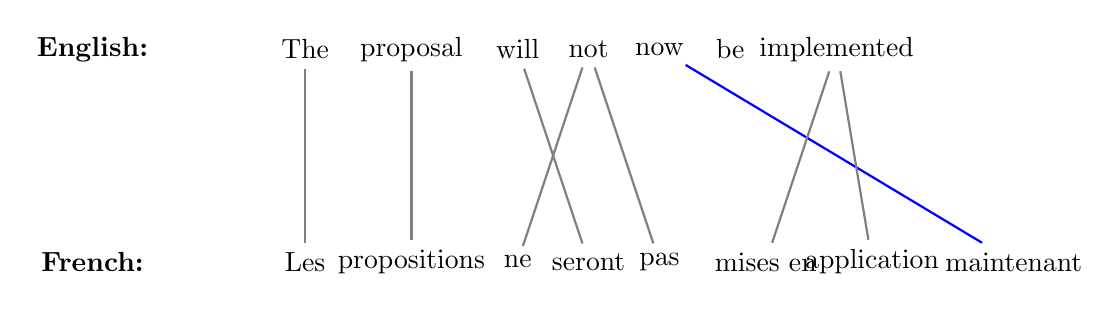
\begin{tikzpicture}[scale=0.9]
        % English sentence
        \node at (-3, 2) {\textbf{English:}};
        \node (e1) at (0, 2) {The};
        \node (e2) at (1.5, 2) {proposal};
        \node (e3) at (3, 2) {will};
        \node (e4) at (4, 2) {not};
        \node (e5) at (5, 2) {now};
        \node (e6) at (6, 2) {be};
        \node (e7) at (7.5, 2) {implemented};

        % French sentence
        \node at (-3, -1) {\textbf{French:}};
        \node (f1) at (0, -1) {Les};
        \node (f2) at (1.5, -1) {propositions};
        \node (f3) at (3, -1) {ne};
        \node (f4) at (4, -1) {seront};
        \node (f5) at (5, -1) {pas};
        \node (f6) at (6.5, -1) {mises en};
        \node (f7) at (8, -1) {application};
        \node (f8) at (10, -1) {maintenant};

        % Alignment lines (showing non-monotonic alignment)
        \draw[-, gray, thick] (e1) -- (f1);
        \draw[-, gray, thick] (e2) -- (f2);
        \draw[-, gray, thick] (e3) -- (f4);
        \draw[-, gray, thick] (e4) -- (f3);
        \draw[-, gray, thick] (e4) -- (f5);
        \draw[-, blue, thick] (e5) -- (f8);  % Crossing alignment
        \draw[-, gray, thick] (e7) -- (f6);
        \draw[-, gray, thick] (e7) -- (f7);
    \end{tikzpicture}
    \caption{Word alignment between English and French (adapted from Brown et al., 1990). Note the crossing alignments: ``now'' at position 5 in English maps to ``maintenant'' at position 9 in French (shown in blue), while ``implemented'' maps to a multi-word phrase. The negation ``not'' maps to the French discontinuous negation ``ne...pas''. These non-monotonic alignments are a key challenge in machine translation.}
    \label{fig:word-alignment}
\end{figure}

This figure reveals several important phenomena:
\begin{itemize}
    \item \textbf{Crossing alignments:} The line from ``now'' to ``maintenant'' crosses other alignment lines, indicating word order changes.
    \item \textbf{One-to-many mapping:} ``implemented'' maps to ``mises en application'' (three French words).
    \item \textbf{Discontinuous alignment:} ``not'' maps to ``ne...pas'', a discontinuous negation construction in French.
\end{itemize}

A model that simply processes the input left-to-right and generates output left-to-right cannot easily handle these phenomena. It would need to ``remember'' that ``now'' appeared early in the sentence and output its translation late, while simultaneously tracking the complex multi-word correspondences.

\begin{quickref}[Seq2Seq Applications Beyond Translation]
The encoder-decoder framework applies to any task where input and output are both sequences of potentially different lengths:
\begin{itemize}
    \item \textbf{Question answering:} Input question $\rightarrow$ output answer (``What is the capital of France?'' $\rightarrow$ ``Paris'')
    \item \textbf{Dialogue systems:} User utterance $\rightarrow$ system response (chatbots, virtual assistants)
    \item \textbf{Text summarisation:} Long document $\rightarrow$ concise summary (abstractive summarisation)
    \item \textbf{Code generation:} Natural language description $\rightarrow$ executable code (GitHub Copilot)
    \item \textbf{Speech recognition:} Audio sequence $\rightarrow$ text transcription
    \item \textbf{Image captioning:} Image features $\rightarrow$ descriptive sentence
    \item \textbf{SQL generation:} Natural language query $\rightarrow$ SQL query
\end{itemize}

In each case, the encoder compresses the input into a representation that the decoder expands into the output sequence.
\end{quickref}

\subsection{The Encoder-Decoder Framework}
\label{subsec:enc-dec-framework}

The encoder-decoder architecture addresses variable-length sequence transformation by introducing an intermediate fixed-dimensional representation called the \textbf{context vector}. This is a form of \textbf{representation learning}: the encoder learns to extract the essential information from the input, while the decoder learns to generate appropriate outputs from this compressed representation.

\begin{rigour}[Encoder-Decoder Architecture]
The architecture consists of two neural network components:

\textbf{1. Encoder:} Takes a variable-length input sequence and transforms it into a \textbf{fixed-shape state} (context vector):
\[
\text{Encoder}: (x_1, x_2, \ldots, x_T) \longrightarrow \mathbf{c} \in \mathbb{R}^h
\]
where $h$ is the hidden dimension (a hyperparameter, typically 256--1024).

\textbf{2. Decoder:} Takes the fixed-shape context and generates a variable-length output sequence:
\[
\text{Decoder}: \mathbf{c} \longrightarrow (y_1, y_2, \ldots, y_{T'})
\]

\textbf{Information flow:}
\[
\underbrace{(x_1, \ldots, x_T)}_{\text{Variable length } T} \xrightarrow{\text{Encoder}} \underbrace{\mathbf{c}}_{\text{Fixed dimension } h} \xrightarrow{\text{Decoder}} \underbrace{(y_1, \ldots, y_{T'})}_{\text{Variable length } T'}
\]

The context vector $\mathbf{c}$ acts as an \textbf{information bottleneck}: it must contain everything the decoder needs to generate the output, compressed into a fixed number of dimensions. This compression forces the encoder to learn a meaningful representation of the input.
\end{rigour}

\begin{figure}[H]
    \centering
    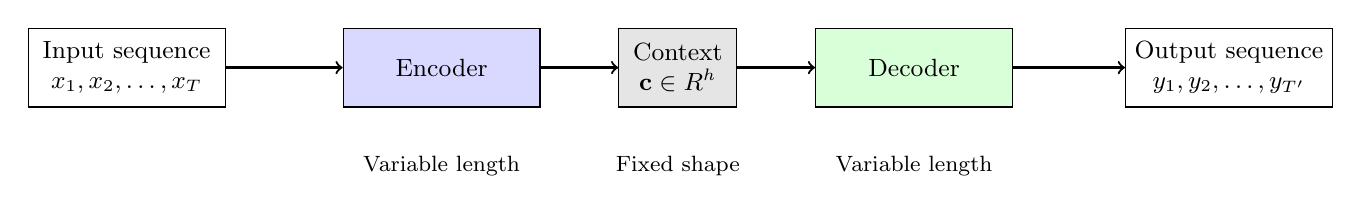
\begin{tikzpicture}[
        box/.style={rectangle, draw, minimum width=2.5cm, minimum height=1cm, align=center, font=\small},
        state/.style={rectangle, draw, fill=gray!20, minimum width=1.5cm, minimum height=1cm, align=center, font=\small},
        arrow/.style={->, thick}
    ]
        \node[box] (input) at (0, 0) {Input sequence\\$x_1, x_2, \ldots, x_T$};
        \node[box, fill=blue!15] (encoder) at (4, 0) {Encoder};
        \node[state] (context) at (7, 0) {Context\\$\mathbf{c} \in \mathbb{R}^h$};
        \node[box, fill=green!15] (decoder) at (10, 0) {Decoder};
        \node[box] (output) at (14, 0) {Output sequence\\$y_1, y_2, \ldots, y_{T'}$};

        \draw[arrow] (input) -- (encoder);
        \draw[arrow] (encoder) -- (context);
        \draw[arrow] (context) -- (decoder);
        \draw[arrow] (decoder) -- (output);

        \node[below=0.3cm] at (4, -0.7) {\footnotesize Variable length};
        \node[below=0.3cm] at (7, -0.7) {\footnotesize Fixed shape};
        \node[below=0.3cm] at (10, -0.7) {\footnotesize Variable length};
    \end{tikzpicture}
    \caption{Encoder-decoder architecture: the encoder compresses a variable-length input into a fixed-dimensional context vector, which the decoder expands into a variable-length output. The context vector is the only pathway for information from input to output-a bottleneck that will prove problematic for long sequences.}
    \label{fig:encoder-decoder-flow}
\end{figure}

\textbf{Why this architecture?} The key insight is that by separating encoding and decoding, we can handle variable-length inputs and outputs independently. The encoder does not need to know how long the output will be; it simply produces the best possible representation of the input. The decoder does not need to know how long the input was; it generates output based solely on the context vector. This modularity makes the architecture flexible and trainable.

\textbf{The bottleneck problem:} However, this flexibility comes at a cost. The context vector $\mathbf{c}$ has fixed dimension $h$ regardless of input length $T$. A 5-word sentence and a 50-word paragraph must both be compressed into the same $h$-dimensional vector. For long sequences, crucial information may be lost in this compression. As we will see, attention mechanisms address precisely this limitation.

\subsection{Autoencoder: A Special Case}
\label{subsec:autoencoder}

Before examining RNN-based seq2seq models, it is instructive to consider a special case: the \textbf{autoencoder}. When the source and target domains are identical-when we want the output to match the input-the encoder-decoder becomes an autoencoder. This seemingly trivial task (reproducing the input) is actually useful for learning compressed representations.

\begin{rigour}[Autoencoder]
\textbf{Definition:} An autoencoder is an encoder-decoder where the target output equals the input:
\[
\text{Autoencoder}: \mathbf{x} \xrightarrow{\text{Encoder } f} \mathbf{z} \xrightarrow{\text{Decoder } g} \hat{\mathbf{x}} \approx \mathbf{x}
\]

The intermediate representation $\mathbf{z}$ (called the \textbf{latent code} or \textbf{bottleneck representation}) typically has lower dimensionality than $\mathbf{x}$, forcing the model to learn a compressed representation that retains the information needed for reconstruction.

\textbf{Training objective:} Minimise reconstruction error:
\[
\mathcal{L}(\theta) = \sum_{i=1}^{N} \|\mathbf{x}^{(i)} - g(f(\mathbf{x}^{(i)}))\|^2 = \sum_{i=1}^{N} \|\mathbf{x}^{(i)} - \hat{\mathbf{x}}^{(i)}\|^2
\]
where $\theta$ denotes all parameters of both encoder and decoder.

\textbf{Architectural constraint:} If $\mathbf{x} \in \mathbb{R}^d$ and $\mathbf{z} \in \mathbb{R}^k$ with $k < d$, the autoencoder forms a \textbf{bottleneck}. The model cannot simply memorise the input; it must learn to extract the most important features.

\textbf{Connection to PCA:} A linear autoencoder (with linear encoder $f(\mathbf{x}) = \mathbf{W}_e \mathbf{x}$ and linear decoder $g(\mathbf{z}) = \mathbf{W}_d \mathbf{z}$) learns the same subspace as PCA. The latent code $\mathbf{z}$ spans the principal component subspace. Nonlinear autoencoders can learn more complex, nonlinear manifolds.
\end{rigour}

\begin{quickref}[Autoencoder Variants and Applications]
\textbf{Variants:}
\begin{itemize}
    \item \textbf{Undercomplete autoencoder:} Bottleneck dimension $k < d$ forces compression (standard case)
    \item \textbf{Overcomplete autoencoder:} Bottleneck dimension $k > d$ with regularisation (sparse autoencoders)
    \item \textbf{Denoising autoencoder:} Input is corrupted; model learns to reconstruct clean version. Trained on pairs $(\tilde{\mathbf{x}}, \mathbf{x})$ where $\tilde{\mathbf{x}}$ is a noisy version of $\mathbf{x}$.
    \item \textbf{Variational autoencoder (VAE):} Imposes probabilistic structure on $\mathbf{z}$ (e.g., $\mathbf{z} \sim \mathcal{N}(\boldsymbol{\mu}, \boldsymbol{\sigma}^2)$), enabling generation of new samples.
    \item \textbf{Contractive autoencoder:} Penalises the Jacobian of the encoder, learning representations robust to small input perturbations.
\end{itemize}

\textbf{Applications:}
\begin{itemize}
    \item \textbf{Dimensionality reduction:} Nonlinear alternative to PCA
    \item \textbf{Anomaly detection:} High reconstruction error indicates the input differs from training distribution
    \item \textbf{Image denoising and compression:} Learn to remove noise or compress images
    \item \textbf{Pretraining:} Learn useful representations before supervised fine-tuning
    \item \textbf{Generative modelling:} VAEs can generate new samples by sampling from the latent space
\end{itemize}
\end{quickref}

The autoencoder illustrates a key principle of encoder-decoder architectures: the bottleneck forces learning. By constraining information flow through a lower-dimensional representation, we force the model to discover the essential structure in the data. In seq2seq models for translation, the analogous constraint forces the encoder to extract meaning that generalises across input lengths.

\subsection{RNN-Based Encoder-Decoder}
\label{subsec:rnn-encoder-decoder}

The natural implementation of encoder-decoder for sequences uses recurrent neural networks (RNNs), as introduced in Week 6. RNNs process sequences token by token, maintaining a hidden state that accumulates information. This makes them well-suited for encoding variable-length sequences into fixed-dimensional representations.

\begin{rigour}[RNN Encoder]
Given an input sequence of tokens $x_1, x_2, \ldots, x_T$, the encoder RNN processes each token sequentially, updating its hidden state:
\[
\mathbf{h}_t = f(\mathbf{x}_t, \mathbf{h}_{t-1})
\]
where:
\begin{itemize}
    \item $\mathbf{h}_t \in \mathbb{R}^h$ is the hidden state at time $t$, summarising all information from $x_1, \ldots, x_t$
    \item $\mathbf{x}_t \in \mathbb{R}^d$ is the embedding of token $x_t$ (see Week 7 on word embeddings)
    \item $f$ is the recurrent function (vanilla RNN, LSTM, or GRU cell-see Week 6)
    \item $\mathbf{h}_0 \in \mathbb{R}^h$ is typically initialised to zeros
\end{itemize}

The encoder transforms the sequence of hidden states into a \textbf{context variable} via a function $q$:
\[
\mathbf{c} = q(\mathbf{h}_1, \mathbf{h}_2, \ldots, \mathbf{h}_T)
\]

\textbf{Simple choice (Sutskever et al., 2014):} Use only the final hidden state:
\[
\mathbf{c} = \mathbf{h}_T
\]

This is computationally simple but problematic for long sequences: information from early tokens must survive $T$ recurrent steps to influence the context. Even with LSTMs, this leads to information loss.

\textbf{Alternative choices for $q$:}
\begin{itemize}
    \item Concatenate final forward and backward hidden states (bidirectional RNN)
    \item Average or max-pool over all hidden states
    \item Use attention over hidden states (leading to the mechanisms we will study)
\end{itemize}
\end{rigour}

\textbf{Why LSTMs/GRUs?} As discussed in Week 6, vanilla RNNs suffer from vanishing gradients that prevent learning long-range dependencies. For machine translation, where a word at the beginning of a long sentence may be crucial for words at the end of the translation, this is particularly problematic. LSTMs and GRUs mitigate (but do not eliminate) this issue through gating mechanisms. The move to attention will provide a more fundamental solution.

\begin{rigour}[RNN Decoder]
Given the context $\mathbf{c}$ and target sequence $y_1, y_2, \ldots, y_{T'}$, the decoder generates output tokens \textbf{autoregressively}-each token is predicted based on all previous tokens.

At each time step $t'$, the decoder:
\begin{enumerate}
    \item Computes a hidden state using the previous token embedding, context, and previous hidden state:
    \[
    \mathbf{s}_{t'} = g(y_{t'-1}, \mathbf{c}, \mathbf{s}_{t'-1})
    \]
    where $g$ is the decoder's recurrent function.

    \item Computes output logits via a linear transformation:
    \[
    \mathbf{o}_{t'} = \mathbf{W}_o \mathbf{s}_{t'} + \mathbf{b}_o \in \mathbb{R}^{|\mathcal{V}|}
    \]
    where $|\mathcal{V}|$ is the vocabulary size.

    \item Applies softmax to get a probability distribution over the vocabulary:
    \[
    P(y_{t'} = v \mid y_1, \ldots, y_{t'-1}, \mathbf{c}) = \frac{\exp(o_{t',v})}{\sum_{v'=1}^{|\mathcal{V}|} \exp(o_{t',v'})}
    \]
\end{enumerate}

\textbf{Implementation details:}
\begin{itemize}
    \item \textbf{Initialisation:} The encoder's final hidden state $\mathbf{h}_T$ initialises the decoder's hidden state: $\mathbf{s}_0 = \mathbf{h}_T$
    \item \textbf{Context injection:} The context $\mathbf{c}$ is concatenated with the input embedding at \textit{every} time step: the decoder input is $[\mathbf{y}_{t'-1}; \mathbf{c}]$
    \item \textbf{Start token:} The first decoder input is a special \texttt{<bos>} (beginning of sequence) token
    \item \textbf{Termination:} Generation stops when the decoder predicts \texttt{<eos>} (end of sequence)
\end{itemize}
\end{rigour}

\begin{figure}[H]
    \centering
    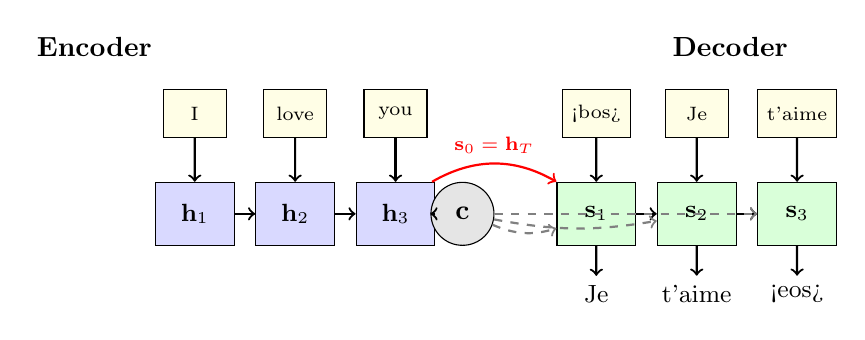
\begin{tikzpicture}[
        rnn/.style={rectangle, draw, fill=blue!15, minimum width=1cm, minimum height=0.8cm, font=\small},
        dec/.style={rectangle, draw, fill=green!15, minimum width=1cm, minimum height=0.8cm, font=\small},
        embed/.style={rectangle, draw, fill=yellow!10, minimum width=0.8cm, minimum height=0.6cm, font=\scriptsize},
        arrow/.style={->, thick},
        scale=0.85
    ]
        % Encoder
        \node at (-4, 2.5) {\textbf{Encoder}};
        \foreach \i/\w in {1/I, 2/love, 3/you} {
            \node[embed] (e\i) at (\i*1.5 - 4, 1.5) {\w};
            \node[rnn] (h\i) at (\i*1.5 - 4, 0) {$\mathbf{h}_\i$};
            \draw[arrow] (e\i) -- (h\i);
        }
        \draw[arrow] (h1) -- (h2);
        \draw[arrow] (h2) -- (h3);

        % Context
        \node[draw, fill=gray!20, circle, minimum size=0.8cm] (c) at (1.5, 0) {$\mathbf{c}$};
        \draw[arrow] (h3) -- (c);

        % Decoder
        \node at (5.5, 2.5) {\textbf{Decoder}};
        \foreach \i/\w in {1/<bos>, 2/Je, 3/t'aime} {
            \node[embed] (d\i) at (\i*1.5 + 2, 1.5) {\w};
            \node[dec] (s\i) at (\i*1.5 + 2, 0) {$\mathbf{s}_\i$};
            \draw[arrow] (d\i) -- (s\i);
        }
        \draw[arrow] (s1) -- (s2);
        \draw[arrow] (s2) -- (s3);

        % Context to all decoder states
        \draw[arrow, dashed, gray] (c) to[bend right=20] (s1);
        \draw[arrow, dashed, gray] (c) to[bend right=10] (s2);
        \draw[arrow, dashed, gray] (c) -- (s3);

        % Outputs
        \foreach \i/\w in {1/Je, 2/t'aime, 3/<eos>} {
            \node[font=\small] (o\i) at (\i*1.5 + 2, -1.2) {\w};
            \draw[arrow] (s\i) -- (o\i);
        }

        % Initial state transfer
        \draw[arrow, thick, red] (h3) to[bend left=30] node[above, font=\scriptsize] {$\mathbf{s}_0 = \mathbf{h}_T$} (s1.north west);
    \end{tikzpicture}
    \caption{RNN encoder-decoder for translating ``I love you'' to French. The encoder processes the English sentence left-to-right, producing hidden states $\mathbf{h}_1, \mathbf{h}_2, \mathbf{h}_3$. The final hidden state $\mathbf{h}_3$ initialises the decoder (red arrow) and serves as the context $\mathbf{c}$. The context is fed to the decoder at every time step (dashed grey arrows). The decoder generates autoregressively: each output becomes the next input.}
    \label{fig:rnn-enc-dec}
\end{figure}

\begin{redbox}
\textbf{Training vs Inference Discrepancy: Teacher Forcing and Exposure Bias}

A critical subtlety arises in how RNN decoders are trained versus how they are used at inference time.

\textbf{During training (teacher forcing):}
\begin{itemize}
    \item The \textbf{ground truth} token $y_{t'-1}$ is fed as input at time $t'$
    \item This is called \textbf{teacher forcing}-the model is ``told'' the correct previous token regardless of what it would have predicted
    \item Enables efficient parallel training: we can compute all losses in parallel since the input at each step is known
    \item Provides stable gradients: the model always sees correct context
\end{itemize}

\textbf{During inference (autoregressive generation):}
\begin{itemize}
    \item The \textbf{predicted} token $\hat{y}_{t'-1}$ is fed as input at time $t'$
    \item The model must use its own (potentially wrong) predictions
    \item Errors compound: a wrong prediction leads to unfamiliar context, leading to more errors
    \item The model never saw its own mistakes during training
\end{itemize}

This train-test mismatch is called \textbf{exposure bias}. The model is ``exposed'' only to ground-truth sequences during training, never to the kind of erroneous sequences it will encounter during inference. This can significantly degrade performance, particularly for long sequences where early errors propagate.

\textbf{Mitigation strategies:}
\begin{itemize}
    \item \textbf{Scheduled sampling:} During training, sometimes use predicted tokens instead of ground truth, with increasing probability over time
    \item \textbf{Beam search:} At inference, maintain multiple hypotheses rather than greedily committing to one prediction
    \item \textbf{Reinforcement learning:} Train with sequence-level rewards (e.g., BLEU score) that account for end-to-end generation quality
\end{itemize}
\end{redbox}

\subsection{Bidirectional Encoding}
\label{subsec:bidirectional}

A limitation of the forward-only encoder is that $\mathbf{h}_t$ only contains information from tokens $x_1, \ldots, x_t$-it cannot incorporate future context. For translation, knowing what comes \textit{after} a word can be just as important as knowing what comes before.

\begin{quickref}[Bidirectional RNN Encoder]
\textbf{Idea:} Process the input sequence in both directions and combine the results.

\textbf{Forward RNN:} Processes $x_1 \rightarrow x_2 \rightarrow \cdots \rightarrow x_T$, producing hidden states $\overrightarrow{\mathbf{h}}_1, \ldots, \overrightarrow{\mathbf{h}}_T$.

\textbf{Backward RNN:} Processes $x_T \rightarrow x_{T-1} \rightarrow \cdots \rightarrow x_1$, producing hidden states $\overleftarrow{\mathbf{h}}_T, \ldots, \overleftarrow{\mathbf{h}}_1$.

\textbf{Combined representation:} At each position $t$, concatenate forward and backward states:
\[
\mathbf{h}_t = [\overrightarrow{\mathbf{h}}_t; \overleftarrow{\mathbf{h}}_t] \in \mathbb{R}^{2h}
\]

Now $\mathbf{h}_t$ contains information from the \textit{entire} sequence, not just the prefix.

\textbf{Context vector options:}
\begin{itemize}
    \item Concatenate final states: $\mathbf{c} = [\overrightarrow{\mathbf{h}}_T; \overleftarrow{\mathbf{h}}_1]$
    \item Average all bidirectional hidden states
    \item Use attention over all $\mathbf{h}_t$ (Bahdanau attention, covered later)
\end{itemize}
\end{quickref}

Bidirectional encoding is standard in modern seq2seq models. It doubles the hidden dimension (or equivalently, uses half the per-direction dimension) but provides much richer representations. The encoder in the original Bahdanau attention model was bidirectional.

\subsection{Data Preprocessing for Machine Translation}
\label{subsec:preprocessing}

Before training translation models, significant preprocessing is required. The choices made here affect model performance considerably.

\begin{quickref}[Machine Translation Preprocessing Pipeline]
\textbf{Data sources:} Parallel corpora-collections of aligned sentence pairs across languages. Examples include:
\begin{itemize}
    \item \textbf{Europarl:} European Parliament proceedings in 21 languages
    \item \textbf{WMT datasets:} Standard benchmarks for machine translation
    \item \textbf{Tatoeba:} Community-contributed sentence pairs for many language pairs
    \item \textbf{OPUS:} Collection of translated texts from the web
\end{itemize}

\textbf{Tokenisation:} Convert text to tokens (see Week 7 for details):
\begin{itemize}
    \item Word-level: Simple but large vocabulary, out-of-vocabulary problem
    \item \textbf{Subword (BPE, WordPiece):} Modern standard; handles rare words gracefully
    \item Character-level: Very long sequences, rarely used alone
\end{itemize}

\textbf{Vocabulary construction:}
\begin{itemize}
    \item Typically 30,000--50,000 subword tokens per language
    \item Shared vocabulary for related languages can improve transfer
    \item Vocabulary must be fixed before training
\end{itemize}
\end{quickref}

\begin{rigour}[Minibatch Construction for Variable-Length Sequences]
Since sentences have variable lengths, batching requires careful handling:

\textbf{1. Truncation:} Keep only the first $L$ tokens; discard the rest
\[
(x_1, x_2, \ldots, x_T) \rightarrow (x_1, x_2, \ldots, x_{\min(T,L)})
\]
This loses information from long sentences but ensures bounded computation.

\textbf{2. Padding:} Append special \texttt{<pad>} tokens to reach length $L$
\[
(x_1, \ldots, x_T) \rightarrow (x_1, \ldots, x_T, \texttt{<pad>}, \ldots, \texttt{<pad>})
\]
This enables batched computation but wastes computation on padding tokens.

\textbf{Special tokens:}
\begin{itemize}
    \item \texttt{<pad>}: Padding for batch alignment (index 0, ignored in loss computation)
    \item \texttt{<bos>}: Beginning of sequence (decoder start signal)
    \item \texttt{<eos>}: End of sequence (signals completion)
    \item \texttt{<unk>}: Unknown/out-of-vocabulary tokens (rare with subword tokenisation)
\end{itemize}

\textbf{Padding masks:} When computing loss or attention, padding tokens must be masked out. The loss function should ignore predictions at padding positions. Attention should not attend to padding tokens.

\textbf{Bucketing:} Group sentences of similar length into the same batches to minimise wasted padding computation. Sort dataset by length, then create batches from consecutive sentences.
\end{rigour}

%==============================================================================
\section{BLEU: Evaluating Machine Translation}
\label{sec:bleu}
%==============================================================================

How do we know if a machine translation system is any good? This is surprisingly difficult to answer. Translation is not a deterministic mapping-there are often multiple valid translations for any source sentence, and human judgement of quality is subjective and expensive.

The BLEU (Bilingual Evaluation Understudy) metric, introduced by Papineni et al.\ (2002), provides an automatic evaluation method that correlates reasonably well with human judgement. Despite its known limitations, BLEU remains the standard metric for comparing translation systems and tracking progress during development.

\subsection{The Challenge of Evaluation}
\label{subsec:eval-challenge}

Consider the English sentence ``The cat sat on the mat.'' Multiple German translations are acceptable:
\begin{itemize}
    \item ``Die Katze sa\ss{} auf der Matte.''
    \item ``Die Katze hat auf der Matte gesessen.''
    \item ``Auf der Matte sa\ss{} die Katze.''
\end{itemize}

Each captures the meaning correctly, though with different word choices, word order, and tense. A good metric must give credit for all valid translations, not just exact matches to a single reference. Simultaneously, it must penalise translations that miss the meaning or include spurious content.

\begin{rigour}[BLEU Score]
\textbf{BLEU (Bilingual Evaluation Understudy)} compares predicted sequences against one or more reference translations using n-gram precision.

\textbf{N-gram precision $p_n$:} The ratio of n-grams in the prediction that also appear in the reference:
\[
p_n = \frac{\text{Number of n-grams in prediction matching any reference}}{\text{Total n-grams in prediction}}
\]

\textbf{Clipped counts:} To prevent gaming the metric by repeating common n-grams, each n-gram match is clipped to its maximum count in the reference. If the reference contains ``the cat'' once, the prediction only gets credit for one ``the cat'' match, even if it contains ``the cat'' five times.

\textbf{BLEU formula:}
\[
\text{BLEU} = \underbrace{\exp\left(\min\left(0, 1 - \frac{\text{len}_{\text{ref}}}{\text{len}_{\text{pred}}}\right)\right)}_{\text{Brevity penalty (BP)}} \cdot \underbrace{\prod_{n=1}^{N} p_n^{w_n}}_{\text{Geometric mean of n-gram precisions}}
\]

where:
\begin{itemize}
    \item $\text{len}_{\text{ref}}$ = number of tokens in reference sequence
    \item $\text{len}_{\text{pred}}$ = number of tokens in predicted sequence
    \item $N$ = maximum n-gram length to consider (typically 4)
    \item $p_n$ = clipped precision of n-grams of length $n$
    \item $w_n$ = weight for n-gram precision (typically $w_n = 1/N = 0.25$)
\end{itemize}

\textbf{Standard configuration:} $N=4$ with uniform weights $w_n = 0.25$ for $n \in \{1,2,3,4\}$.
\end{rigour}

Let us unpack each component of the BLEU formula:

\textbf{1. N-gram precision:} The core idea is that good translations share n-grams with references. Unigram precision measures how many words in the prediction appear in the reference. Bigram precision measures how many word pairs appear. Higher-order n-grams capture phrase-level and sentence-level structure.

\textbf{2. Geometric mean:} Using the geometric mean (rather than arithmetic) means that if \textit{any} n-gram precision is zero, the entire BLEU score is zero. This ensures that a translation must match at all n-gram levels to score well.

\textbf{3. Brevity penalty (BP):} Without this, a system could achieve high precision by outputting only a single confident word. The BP penalises translations shorter than the reference:
\[
\text{BP} = \begin{cases}
1 & \text{if } \text{len}_{\text{pred}} \geq \text{len}_{\text{ref}} \\
\exp\left(1 - \frac{\text{len}_{\text{ref}}}{\text{len}_{\text{pred}}}\right) & \text{otherwise}
\end{cases}
\]

Note: The formula in the original notes uses $\min(0, 1 - \text{len}_{\text{label}}/\text{len}_{\text{pred}})$, which is equivalent-it equals zero when prediction is longer (giving BP = 1), and is negative otherwise.

\begin{quickref}[BLEU Score Properties]
\textbf{Range:} BLEU $\in [0, 1]$, with 1 indicating perfect match to reference(s).

\textbf{Interpretation guidelines} (for news translation):
\begin{itemize}
    \item $<$ 0.10: Almost useless
    \item 0.10--0.20: Gist is understandable
    \item 0.20--0.30: Reasonable quality
    \item 0.30--0.40: High quality
    \item 0.40--0.50: Very high quality
    \item $>$ 0.50: Exceptional (approaching human)
\end{itemize}

\textbf{Key properties:}
\begin{itemize}
    \item \textbf{Precision-based:} Measures what fraction of predicted n-grams are correct
    \item \textbf{Multiple references:} Can use multiple valid translations; match to any counts
    \item \textbf{Corpus-level:} Best computed over many sentences; sentence-level BLEU is noisy
    \item \textbf{Case-sensitive:} Standard BLEU distinguishes ``The'' from ``the''
\end{itemize}
\end{quickref}

\begin{rigour}[BLEU Worked Example]
Consider:
\begin{itemize}
    \item \textbf{Reference:} ``the cat sat on the mat'' (6 tokens)
    \item \textbf{Prediction:} ``the cat on the mat'' (5 tokens)
\end{itemize}

The prediction is missing ``sat'' but otherwise matches.

\textbf{Step 1: Compute unigram precision ($p_1$):}
\begin{itemize}
    \item Prediction unigrams: \{the, cat, on, the, mat\}
    \item Reference unigrams: \{the, cat, sat, on, the, mat\}
    \item All 5 prediction unigrams appear in reference
    \item $p_1 = 5/5 = 1.0$
\end{itemize}

\textbf{Step 2: Compute bigram precision ($p_2$):}
\begin{itemize}
    \item Prediction bigrams: \{the-cat, cat-on, on-the, the-mat\} (4 bigrams)
    \item Reference bigrams: \{the-cat, cat-sat, sat-on, on-the, the-mat\} (5 bigrams)
    \item Matches: the-cat, on-the, the-mat (3 matches)
    \item Missing: cat-on (the reference has cat-sat, not cat-on)
    \item $p_2 = 3/4 = 0.75$
\end{itemize}

\textbf{Step 3: Compute brevity penalty:}
\[
\text{BP} = \exp\left(\min\left(0, 1 - \frac{6}{5}\right)\right) = \exp\left(\min(0, -0.2)\right) = \exp(-0.2) \approx 0.819
\]
The prediction is shorter than the reference, so the BP $< 1$.

\textbf{Step 4: Compute BLEU (using $N=2$ for simplicity):}

With uniform weights $w_1 = w_2 = 0.5$:
\[
\text{BLEU} = 0.819 \times (1.0)^{0.5} \times (0.75)^{0.5} = 0.819 \times 1.0 \times 0.866 \approx 0.71
\]

\textbf{Interpretation:} Despite missing one word, the translation scores 0.71 because most n-grams match. The brevity penalty reduces the score by about 18\% due to the shorter length.
\end{rigour}

\begin{redbox}
\textbf{BLEU Limitations}

Despite its widespread use, BLEU has significant limitations:

\textbf{1. No semantic awareness:}
\begin{itemize}
    \item ``I love dogs'' vs ``I adore canines'' share no 2+-grams, but mean the same thing
    \item Synonyms and paraphrases receive no credit
\end{itemize}

\textbf{2. Order insensitivity beyond n-grams:}
\begin{itemize}
    \item ``John loves Mary'' vs ``Mary loves John'' may have similar BLEU despite different meanings
    \item Only catches order differences within n-gram windows
\end{itemize}

\textbf{3. No fluency guarantee:}
\begin{itemize}
    \item High n-gram overlap does not ensure the translation reads naturally
    \item Grammatical errors may not be penalised if individual n-grams are correct
\end{itemize}

\textbf{4. Short sentence instability:}
\begin{itemize}
    \item For short sentences, a single word mismatch dramatically affects the score
    \item BLEU is more reliable as a corpus-level metric than sentence-level
\end{itemize}

\textbf{5. Reference dependence:}
\begin{itemize}
    \item Score depends heavily on which references are provided
    \item A valid translation absent from references will score poorly
\end{itemize}

\textbf{Modern alternatives:} METEOR (considers synonyms), chrF (character-level), BERTScore (embedding similarity), BLEURT (learned metric), and human evaluation for final assessment.
\end{redbox}

\subsection{Computing BLEU in Practice}

\begin{quickref}[Practical BLEU Computation]
\textbf{Corpus-level BLEU:} Sum n-gram counts across all sentences before computing precision:
\[
p_n = \frac{\sum_{\text{sentences}} \text{clipped n-gram matches}}{\sum_{\text{sentences}} \text{total predicted n-grams}}
\]

\textbf{Smoothing:} For sentence-level BLEU, add small epsilon to avoid zero scores when n-gram precision is zero.

\textbf{Tokenisation:} BLEU score depends on tokenisation. Standard practice:
\begin{itemize}
    \item Use consistent tokenisation for prediction and reference
    \item The \texttt{sacrebleu} library provides standardised BLEU computation
\end{itemize}

\textbf{Reporting:} Always report the exact BLEU configuration (e.g., ``BLEU-4, case-sensitive, sacrebleu tokeniser'') for reproducibility.
\end{quickref}

%==============================================================================
\section{The Attention Mechanism}
\label{sec:attention}
%==============================================================================

We now arrive at the central innovation that transformed deep learning: the attention mechanism. What began as a solution to the information bottleneck problem in machine translation has become the foundation for virtually all state-of-the-art models in NLP, computer vision, and beyond.

The core insight is simple but powerful: instead of compressing the entire input into a single fixed-dimensional vector, allow the model to dynamically focus on different parts of the input for each output decision. This ``selective focus'' mirrors how humans process information-we do not perceive all visual input equally, but rather attend to relevant regions based on our current task.

\subsection{The Problem: Information Bottleneck}
\label{subsec:bottleneck}

Before introducing attention, let us understand precisely what problem it solves.

\begin{redbox}
\textbf{The Long Sequence Problem}

In vanilla RNN encoder-decoder models, the entire input sequence must pass through a single bottleneck:

\begin{itemize}
    \item Only the \textbf{final hidden state} $\mathbf{h}_T$ is passed to the decoder as the context
    \item The entire input sequence-no matter how long-must be compressed into a single fixed-dimensional vector $\mathbf{c} \in \mathbb{R}^h$
    \item For long sequences, information from early tokens is progressively ``forgotten'' or overwritten
    \item The decoder uses the \textbf{same context} $\mathbf{c}$ regardless of which output token it is generating
\end{itemize}

\textbf{Why this is problematic:}

Not all input tokens are equally relevant to each output token. When translating ``I would like to learn German'':
\begin{itemize}
    \item When generating ``lernen'' (learn), the model should focus on ``learn''
    \item When generating ``Deutsch'' (German), the model should focus on ``German''
    \item When generating ``m\"{o}chte'' (would like), the model should focus on ``would like''
\end{itemize}

But with a single fixed context $\mathbf{c}$, all this information is jumbled together. The decoder cannot ``look back'' to find the relevant source word.

\textbf{Empirical evidence:} Sutskever et al.\ (2014) found that translation quality degraded significantly for sentences longer than about 20 words. Reversing the input sequence helped (putting recent words closer to the decoder), but this was a band-aid, not a solution.
\end{redbox}

The information bottleneck becomes more intuitive with a concrete example. Imagine you are translating a 50-word paragraph. The encoder produces hidden states $\mathbf{h}_1, \mathbf{h}_2, \ldots, \mathbf{h}_{50}$, each containing information about the sequence up to that point. But only $\mathbf{h}_{50}$ is passed to the decoder. This single vector must somehow encode the meaning of all 50 words in a way that allows the decoder to produce a correct translation of potentially different length.

This is akin to reading a paragraph and then trying to summarise it while blindfolded-you have a single mental representation that must serve all your summarisation needs. Attention lets you ``look back'' at the original text while writing each word of the summary.

\subsection{Biological Inspiration: How Humans Attend}
\label{subsec:bio-inspiration}

The attention mechanism draws inspiration from human visual and cognitive attention. Understanding this biological motivation provides intuition for why attention works.

\begin{quickref}[Attention in Biological Systems]
\textbf{The problem of information overload:}
\begin{itemize}
    \item The human retina has approximately 130 million photoreceptors
    \item The optic nerve transmits roughly $10^6$ bits per second
    \item The brain cannot fully process all incoming visual information in real-time
    \item Similar constraints apply to other sensory modalities
\end{itemize}

\textbf{The solution: selective attention:}
\begin{itemize}
    \item We focus cognitive resources on a small subset of available information
    \item Attention acts as a ``spotlight'' that enhances processing of selected regions
    \item Unattended information is processed superficially or ignored
    \item This allows efficient use of limited cognitive resources
\end{itemize}

\textbf{Key properties of biological attention:}
\begin{itemize}
    \item \textbf{Selective focus:} Concentrate on a fraction of available information
    \item \textbf{Limited capacity:} Attending to one thing means reduced processing of others (opportunity cost)
    \item \textbf{Top-down control:} Attention can be directed voluntarily based on goals
    \item \textbf{Bottom-up capture:} Salient stimuli can capture attention involuntarily
\end{itemize}
\end{quickref}

\begin{rigour}[Types of Attention Cues]
Psychological research distinguishes two types of attention cues, both of which find analogues in neural attention:

\textbf{1. Non-volitional (bottom-up / stimulus-driven) cues:}
\begin{itemize}
    \item Attention captured by \textbf{saliency and conspicuity} of stimuli
    \item Automatic, not requiring conscious effort
    \item Examples: A loud noise captures your attention; a bright red object stands out in a grey scene
    \item In neural networks: Content-based similarity-an unusual or distinctive input pattern draws attention
\end{itemize}

\textbf{2. Volitional (top-down / goal-directed) cues:}
\begin{itemize}
    \item Attention directed based on \textbf{current goals and selection criteria}
    \item Deliberate, requiring cognitive effort
    \item Examples: Searching for your keys; reading a specific paragraph while skimming a page
    \item In neural networks: Query-based retrieval-the decoder's current state determines what to attend to
\end{itemize}

\textbf{Neural attention synthesises both:}
\begin{itemize}
    \item The \textbf{query} represents the volitional cue (what we are looking for)
    \item The \textbf{keys} represent non-volitional cues (what is available and how salient each piece is)
    \item The attention mechanism combines these to determine where to focus
\end{itemize}
\end{rigour}

This biological perspective helps explain why attention is so effective: it mirrors the resource allocation strategy that evolution developed for handling information overload. By selectively attending to relevant inputs, models can effectively have unlimited ``memory'' (access to all inputs) while directing computational resources where they matter most.

\subsection{Queries, Keys, and Values}
\label{subsec:qkv}

The attention mechanism formalises selective focus using three components, inspired by information retrieval systems. This terminology, while initially unfamiliar, provides a powerful framework for understanding attention.

\begin{rigour}[Query-Key-Value Framework]
\textbf{The database analogy:}

Think of attention as querying a database:
\begin{itemize}
    \item You have a \textbf{query}-what you are looking for
    \item The database contains \textbf{key-value pairs}-each record has an identifier (key) and content (value)
    \item You compare your query to all keys to find relevant records
    \item You retrieve a weighted combination of values based on query-key similarity
\end{itemize}

\textbf{Formal definitions:}
\begin{itemize}
    \item \textbf{Query} ($\mathbf{q} \in \mathbb{R}^{d_q}$): What we are looking for; represents the current decoder state or position
    \item \textbf{Keys} ($\mathbf{k}_1, \ldots, \mathbf{k}_n \in \mathbb{R}^{d_k}$): Identifiers for each piece of available information; represent encoder positions
    \item \textbf{Values} ($\mathbf{v}_1, \ldots, \mathbf{v}_n \in \mathbb{R}^{d_v}$): The actual information content to retrieve; typically the encoder hidden states
\end{itemize}

\textbf{Structure:} Each value is paired with a key: $\{(\mathbf{k}_1, \mathbf{v}_1), (\mathbf{k}_2, \mathbf{v}_2), \ldots, (\mathbf{k}_n, \mathbf{v}_n)\}$.

\textbf{The attention mechanism:}
\begin{enumerate}
    \item \textbf{Score:} Compare query to each key to compute \textbf{attention scores} $e_i = \text{score}(\mathbf{q}, \mathbf{k}_i)$
    \item \textbf{Normalise:} Convert scores to \textbf{attention weights} via softmax: $\alpha_i = \frac{\exp(e_i)}{\sum_{j=1}^{n} \exp(e_j)}$
    \item \textbf{Aggregate:} Compute weighted sum of values: $\text{output} = \sum_{i=1}^{n} \alpha_i \mathbf{v}_i$
\end{enumerate}

\textbf{Intuition:} The query ``asks a question'' about what information is needed. Keys determine how relevant each piece of information is to that question. Values provide the actual content. High query-key similarity means the corresponding value contributes more to the output.
\end{rigour}

\begin{figure}[H]
    \centering
    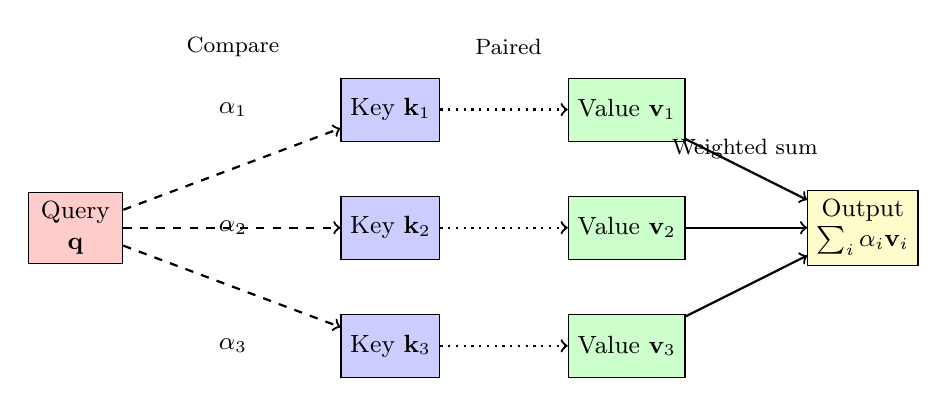
\begin{tikzpicture}[
        query/.style={rectangle, draw, fill=red!20, minimum width=1.2cm, minimum height=0.8cm, align=center, font=\small},
        key/.style={rectangle, draw, fill=blue!20, minimum width=1.2cm, minimum height=0.8cm, align=center, font=\small},
        value/.style={rectangle, draw, fill=green!20, minimum width=1.2cm, minimum height=0.8cm, align=center, font=\small},
        output/.style={rectangle, draw, fill=yellow!20, minimum width=1.2cm, minimum height=0.8cm, align=center, font=\small},
        arrow/.style={->, thick}
    ]
        % Query
        \node[query] (q) at (0, 0) {Query\\$\mathbf{q}$};

        % Keys and Values
        \node[key] (k1) at (4, 1.5) {Key $\mathbf{k}_1$};
        \node[key] (k2) at (4, 0) {Key $\mathbf{k}_2$};
        \node[key] (k3) at (4, -1.5) {Key $\mathbf{k}_3$};

        \node[value] (v1) at (7, 1.5) {Value $\mathbf{v}_1$};
        \node[value] (v2) at (7, 0) {Value $\mathbf{v}_2$};
        \node[value] (v3) at (7, -1.5) {Value $\mathbf{v}_3$};

        % Scores
        \node at (2, 1.5) {\small $\alpha_1$};
        \node at (2, 0) {\small $\alpha_2$};
        \node at (2, -1.5) {\small $\alpha_3$};

        % Output
        \node[output] (out) at (10, 0) {Output\\$\sum_i \alpha_i \mathbf{v}_i$};

        % Arrows from query to keys
        \draw[arrow, dashed] (q) -- (k1);
        \draw[arrow, dashed] (q) -- (k2);
        \draw[arrow, dashed] (q) -- (k3);

        % Arrows from keys to values (pairing)
        \draw[arrow, dotted] (k1) -- (v1);
        \draw[arrow, dotted] (k2) -- (v2);
        \draw[arrow, dotted] (k3) -- (v3);

        % Arrows from values to output
        \draw[arrow] (v1) -- (out);
        \draw[arrow] (v2) -- (out);
        \draw[arrow] (v3) -- (out);

        % Labels
        \node at (2, 2.3) {\footnotesize Compare};
        \node at (5.5, 2.3) {\footnotesize Paired};
        \node at (8.5, 1) {\footnotesize Weighted sum};
    \end{tikzpicture}
    \caption{The query-key-value attention mechanism. The query is compared to all keys to produce attention weights $\alpha_i$ (dashed arrows). Each key is paired with a value (dotted arrows). The output is a weighted sum of values, where weights reflect query-key similarity.}
    \label{fig:qkv-attention}
\end{figure}

\begin{quickref}[Query-Key-Value in Different Contexts]
The Q/K/V terminology unifies several attention variants:

\textbf{Encoder-decoder attention (Bahdanau):}
\begin{itemize}
    \item Query: Decoder hidden state $\mathbf{s}_{t'-1}$ (what output position needs)
    \item Keys \& Values: Encoder hidden states $\mathbf{h}_1, \ldots, \mathbf{h}_T$ (input representations)
\end{itemize}

\textbf{Self-attention (Transformer):}
\begin{itemize}
    \item Query, Keys, Values: All derived from the same sequence
    \item Each position can attend to all positions (including itself)
\end{itemize}

\textbf{Cross-attention (Transformer decoder):}
\begin{itemize}
    \item Query: Decoder representations
    \item Keys \& Values: Encoder representations
\end{itemize}

In all cases, the mechanism is the same: compare queries to keys, weight values accordingly.
\end{quickref}

\textbf{Keys and values: why separate them?} In the simplest case, keys and values are identical (both are the encoder hidden states). But separating them provides flexibility: keys can be optimised for ``findability'' (what makes a position relevant to a query), while values can be optimised for ``information content'' (what information should be retrieved). In Transformers, keys and values are separate linear projections of the same underlying representation.

\subsection{Attention Pooling: From Hard to Soft Retrieval}
\label{subsec:attention-pooling}

Attention can be viewed as a form of \textbf{pooling}-aggregating information from multiple sources into a single output. Unlike average pooling (equal weights) or max pooling (winner-take-all), attention pooling uses learned, input-dependent weights.

\begin{rigour}[Attention Pooling]
\textbf{General form:} Given query $\mathbf{q}$ and key-value pairs $\{(\mathbf{k}_i, \mathbf{v}_i)\}_{i=1}^n$, the attention output is:
\[
\text{Attention}(\mathbf{q}, \{(\mathbf{k}_i, \mathbf{v}_i)\}) = \sum_{i=1}^{n} \alpha(\mathbf{q}, \mathbf{k}_i) \, \mathbf{v}_i
\]
where $\alpha(\mathbf{q}, \mathbf{k}_i) \geq 0$ and $\sum_{i=1}^{n} \alpha(\mathbf{q}, \mathbf{k}_i) = 1$.

The constraint that weights sum to 1 ensures this is a proper weighted average (convex combination) of values.

\textbf{Hard vs soft attention:}
\begin{itemize}
    \item \textbf{Hard attention:} $\alpha_i \in \{0, 1\}$-select exactly one value (non-differentiable; requires reinforcement learning)
    \item \textbf{Soft attention:} $\alpha_i \in [0, 1]$-weighted combination (differentiable; standard practice)
\end{itemize}

Soft attention allows gradient flow through all positions, enabling end-to-end training with backpropagation.
\end{rigour}

To build intuition, consider a classical non-parametric method that can be viewed as attention:

\begin{rigour}[Nadaraya-Watson Kernel Regression as Attention]
\textbf{Problem:} Given training points $\{(x_1, y_1), \ldots, (x_n, y_n)\}$, predict $y$ for a new query point $x$.

\textbf{Kernel regression solution:}
\[
f(x) = \sum_{i=1}^{n} \frac{K(x - x_i)}{\sum_{j=1}^{n} K(x - x_j)} \, y_i = \sum_{i=1}^{n} \alpha(x, x_i) \, y_i
\]

where $K(\cdot)$ is a kernel function (e.g., Gaussian: $K(u) = \exp(-u^2/2)$).

\textbf{Attention interpretation:}
\begin{itemize}
    \item Query: The new input point $x$
    \item Keys: Training inputs $x_1, \ldots, x_n$
    \item Values: Training outputs $y_1, \ldots, y_n$
    \item Attention weights: $\alpha(x, x_i) = \frac{K(x - x_i)}{\sum_j K(x - x_j)}$ (normalised kernel similarities)
\end{itemize}

The prediction is a weighted average of training outputs, with weights determined by similarity to the query. Nearby training points contribute more; distant points contribute less.

\textbf{This is non-parametric attention:} The form of the attention weights is fixed by the kernel choice; there are no learned parameters in the attention mechanism itself (though the kernel bandwidth could be learned).
\end{rigour}

\begin{figure}[H]
    \centering
    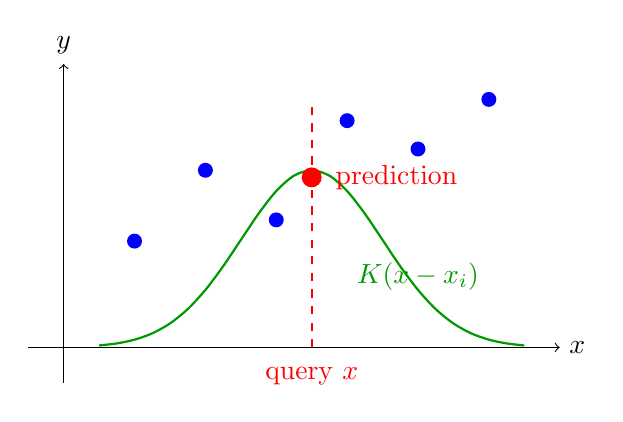
\begin{tikzpicture}[scale=0.9]
        % Axes
        \draw[->] (-0.5, 0) -- (7, 0) node[right] {$x$};
        \draw[->] (0, -0.5) -- (0, 4) node[above] {$y$};

        % Training points
        \foreach \x/\y in {1/1.5, 2/2.5, 3/1.8, 4/3.2, 5/2.8, 6/3.5} {
            \fill[blue] (\x, \y) circle (3pt);
        }

        % Query point
        \draw[red, thick, dashed] (3.5, 0) -- (3.5, 3.5);
        \node[red] at (3.5, -0.4) {query $x$};

        % Kernel illustration
        \draw[green!60!black, thick] plot[smooth, domain=0.5:6.5] (\x, {2.5*exp(-0.5*(\x-3.5)^2)});
        \node[green!60!black] at (5, 1) {$K(x - x_i)$};

        % Weighted average result
        \fill[red] (3.5, 2.4) circle (4pt);
        \node[red, right] at (3.7, 2.4) {prediction};
    \end{tikzpicture}
    \caption{Kernel regression as attention. Training points (blue) have associated $y$ values. For a query point $x$ (red dashed line), the kernel (green curve) assigns weights based on distance. The prediction (red point) is a weighted average of training $y$ values, with nearby points weighted more heavily.}
    \label{fig:kernel-regression}
\end{figure}

\begin{rigour}[Parametric Attention Pooling]
To make attention learnable, we introduce parameters into the attention computation.

\textbf{Parametric kernel example:} With a Gaussian kernel and learnable width $w$:
\[
\alpha(x, x_i) = \text{softmax}\left(-\frac{1}{2}[(x - x_i) \cdot w]^2\right)
\]

The parameter $w$ is learned from data, allowing the model to adapt the ``sharpness'' of attention-how rapidly weights decay with distance.

\textbf{General parametric attention:}
\[
\alpha(\mathbf{q}, \mathbf{k}_i) = \frac{\exp(\text{score}_\theta(\mathbf{q}, \mathbf{k}_i))}{\sum_{j=1}^{n} \exp(\text{score}_\theta(\mathbf{q}, \mathbf{k}_j))}
\]

where $\text{score}_\theta$ is a parameterised scoring function (with learnable parameters $\theta$).

The choice of scoring function is crucial and leads to different attention variants.
\end{rigour}

\subsection{Attention Scoring Functions}
\label{subsec:scoring-functions}

The scoring function determines how query-key similarity is computed. Different choices lead to different computational trade-offs and expressive power. The two main variants are additive (Bahdanau) attention and scaled dot-product attention.

\begin{rigour}[Additive (Bahdanau) Attention]
\textbf{Use case:} When queries and keys have \textbf{different dimensions}: $\mathbf{q} \in \mathbb{R}^{d_q}$, $\mathbf{k} \in \mathbb{R}^{d_k}$, with $d_q \neq d_k$ in general.

\textbf{Scoring function:}
\[
\text{score}(\mathbf{q}, \mathbf{k}) = \mathbf{w}_v^\top \tanh(\mathbf{W}_q \mathbf{q} + \mathbf{W}_k \mathbf{k}) \in \mathbb{R}
\]

\textbf{Learnable parameters:}
\begin{itemize}
    \item $\mathbf{W}_q \in \mathbb{R}^{h \times d_q}$: Projects query to hidden dimension $h$
    \item $\mathbf{W}_k \in \mathbb{R}^{h \times d_k}$: Projects key to hidden dimension $h$
    \item $\mathbf{w}_v \in \mathbb{R}^h$: Maps combined representation to scalar score
\end{itemize}

\textbf{Computation steps:}
\begin{enumerate}
    \item Project query: $\mathbf{q}' = \mathbf{W}_q \mathbf{q} \in \mathbb{R}^h$
    \item Project key: $\mathbf{k}' = \mathbf{W}_k \mathbf{k} \in \mathbb{R}^h$
    \item Add and apply nonlinearity: $\mathbf{a} = \tanh(\mathbf{q}' + \mathbf{k}') \in \mathbb{R}^h$
    \item Project to scalar: $\text{score} = \mathbf{w}_v^\top \mathbf{a} \in \mathbb{R}$
\end{enumerate}

\textbf{Complexity:} $O(h \cdot (d_q + d_k))$ per query-key pair.

\textbf{Why additive?} The query and key projections are \textit{added} (not multiplied), allowing the model to learn attention patterns even when $d_q \neq d_k$. The $\tanh$ nonlinearity allows learning nonlinear relationships.
\end{rigour}

\begin{rigour}[Scaled Dot-Product Attention]
\textbf{Use case:} When queries and keys have the \textbf{same dimension}: $\mathbf{q}, \mathbf{k} \in \mathbb{R}^d$.

\textbf{Scoring function:}
\[
\text{score}(\mathbf{q}, \mathbf{k}) = \frac{\mathbf{q}^\top \mathbf{k}}{\sqrt{d}}
\]

The dot product measures similarity (higher when vectors point in the same direction).

\textbf{Full attention computation:}
\[
\text{Attention}(\mathbf{Q}, \mathbf{K}, \mathbf{V}) = \text{softmax}\left(\frac{\mathbf{Q} \mathbf{K}^\top}{\sqrt{d}}\right) \mathbf{V}
\]

where $\mathbf{Q} \in \mathbb{R}^{m \times d}$, $\mathbf{K} \in \mathbb{R}^{n \times d}$, $\mathbf{V} \in \mathbb{R}^{n \times d_v}$ are matrices with queries, keys, and values as rows.

\textbf{Output dimensions:} The attention output is $\in \mathbb{R}^{m \times d_v}$-one $d_v$-dimensional vector per query.

\textbf{No learnable parameters:} The scoring function itself has no parameters! Learning happens through the linear projections that produce Q, K, V from input representations.
\end{rigour}

\begin{rigour}[Why Scale by $\sqrt{d}$?]
The scaling factor $\sqrt{d}$ is crucial for training stability. Here is why:

\textbf{Problem:} For large $d$, the dot product $\mathbf{q}^\top \mathbf{k}$ can have large magnitude.

\textbf{Statistical analysis:} Assume query and key components are independent with zero mean and unit variance: $q_i, k_i \sim \mathcal{N}(0, 1)$ i.i.d.

The dot product is:
\[
\mathbf{q}^\top \mathbf{k} = \sum_{i=1}^{d} q_i k_i
\]

Each term $q_i k_i$ has:
\begin{itemize}
    \item $\mathbb{E}[q_i k_i] = \mathbb{E}[q_i] \mathbb{E}[k_i] = 0$ (by independence and zero mean)
    \item $\text{Var}(q_i k_i) = \mathbb{E}[q_i^2 k_i^2] - \mathbb{E}[q_i k_i]^2 = \mathbb{E}[q_i^2] \mathbb{E}[k_i^2] = 1$ (since fourth moment of standard normal is 3, but $\mathbb{E}[q_i^2] = \text{Var}(q_i) = 1$)
\end{itemize}

By linearity and independence across $i$:
\[
\mathbb{E}[\mathbf{q}^\top \mathbf{k}] = 0, \quad \text{Var}(\mathbf{q}^\top \mathbf{k}) = d
\]

\textbf{The issue:} For large $d$, dot products have standard deviation $\sqrt{d}$. Some scores will be very large or very small.

When we apply softmax to scores with large variance:
\[
\text{softmax}(e_1, \ldots, e_n)_i = \frac{\exp(e_i)}{\sum_j \exp(e_j)}
\]

If one $e_i$ is much larger than others, softmax ``saturates''-almost all weight goes to one position, gradients become tiny (softmax is nearly flat when saturated), and learning stalls.

\textbf{The solution:} Divide by $\sqrt{d}$ to normalise variance:
\[
\text{Var}\left(\frac{\mathbf{q}^\top \mathbf{k}}{\sqrt{d}}\right) = \frac{\text{Var}(\mathbf{q}^\top \mathbf{k})}{d} = \frac{d}{d} = 1
\]

Now scores have unit variance regardless of $d$, keeping softmax in a well-behaved regime with healthy gradients.
\end{rigour}

\begin{quickref}[Comparison: Additive vs Scaled Dot-Product Attention]
\begin{center}
\begin{tabular}{lcc}
\textbf{Property} & \textbf{Additive} & \textbf{Scaled Dot-Product} \\
\hline
Dimension constraint & $d_q$ and $d_k$ can differ & Requires $d_q = d_k = d$ \\
Learnable parameters & Yes ($\mathbf{W}_q$, $\mathbf{W}_k$, $\mathbf{w}_v$) & No (in scoring function) \\
Nonlinearity & $\tanh$ & None \\
Complexity per pair & $O(h \cdot (d_q + d_k))$ & $O(d)$ \\
GPU efficiency & Moderate & Highly optimised (GEMM) \\
Used in & Bahdanau (2015) & Transformer (2017) \\
\end{tabular}
\end{center}

\textbf{Key insight:} Scaled dot-product attention is simpler, faster, and relies on matrix multiplication-the most optimised operation on modern hardware. This efficiency is crucial for the Transformer's success.

\textbf{Bahdanau et al.\ (2015)} showed that additive and dot-product attention perform similarly, but dot-product is much faster when $d$ is large due to efficient matrix multiplication implementations.
\end{quickref}

\begin{rigour}[Attention Weights as Soft Alignment]
The attention weights $\alpha_{ij}$ can be interpreted as a \textbf{soft alignment} between positions:

\[
\alpha_{ij} = \frac{\exp(\text{score}(\mathbf{q}_i, \mathbf{k}_j))}{\sum_{k=1}^{n} \exp(\text{score}(\mathbf{q}_i, \mathbf{k}_k))}
\]

\textbf{Interpretation:}
\begin{itemize}
    \item $\alpha_{ij}$ represents how much output position $i$ ``aligns with'' or ``attends to'' input position $j$
    \item For each output position $i$, we have a distribution over input positions: $\sum_j \alpha_{ij} = 1$
    \item High $\alpha_{ij}$ means the model considers input position $j$ highly relevant for producing output at position $i$
\end{itemize}

\textbf{Visualisation:} Attention weights can be displayed as a heatmap:
\begin{itemize}
    \item Rows = output positions (queries)
    \item Columns = input positions (keys)
    \item Cell colour = attention weight $\alpha_{ij}$
\end{itemize}

For translation, this often reveals interpretable patterns-when translating a word, the model attends to corresponding source words.
\end{rigour}

\begin{figure}[H]
    \centering
    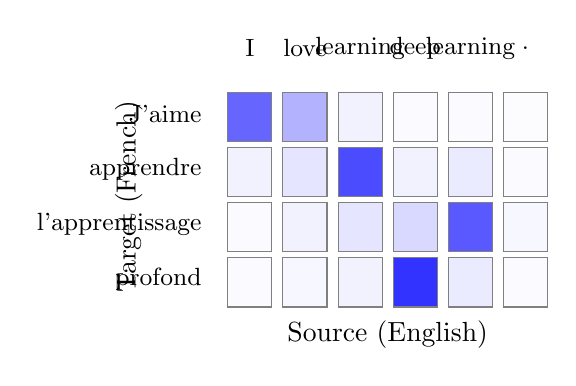
\begin{tikzpicture}[scale=0.7]
        % Grid
        \def\rows{4}
        \def\cols{6}

        % Column labels (source)
        \foreach \j/\w in {1/I, 2/love, 3/learning, 4/deep, 5/learning, 6/.} {
            \node[font=\small] at (\j, \rows + 0.7) {\w};
        }

        % Row labels (target)
        \foreach \i/\w in {1/J'aime, 2/apprendre, 3/l'apprentissage, 4/profond} {
            \node[font=\small, anchor=east] at (0.3, \rows - \i + 0.5) {\w};
        }

        % Attention weights - row 1 (J'aime -> I, love)
        \fill[blue!60!white] (1-0.4, 3) rectangle (1+0.4, 3.9); \draw[gray] (1-0.4, 3) rectangle (1+0.4, 3.9);
        \fill[blue!30!white] (2-0.4, 3) rectangle (2+0.4, 3.9); \draw[gray] (2-0.4, 3) rectangle (2+0.4, 3.9);
        \fill[blue!5!white] (3-0.4, 3) rectangle (3+0.4, 3.9); \draw[gray] (3-0.4, 3) rectangle (3+0.4, 3.9);
        \fill[blue!2!white] (4-0.4, 3) rectangle (4+0.4, 3.9); \draw[gray] (4-0.4, 3) rectangle (4+0.4, 3.9);
        \fill[blue!2!white] (5-0.4, 3) rectangle (5+0.4, 3.9); \draw[gray] (5-0.4, 3) rectangle (5+0.4, 3.9);
        \fill[blue!1!white] (6-0.4, 3) rectangle (6+0.4, 3.9); \draw[gray] (6-0.4, 3) rectangle (6+0.4, 3.9);
        % Row 2 (apprendre -> learning)
        \fill[blue!5!white] (1-0.4, 2) rectangle (1+0.4, 2.9); \draw[gray] (1-0.4, 2) rectangle (1+0.4, 2.9);
        \fill[blue!10!white] (2-0.4, 2) rectangle (2+0.4, 2.9); \draw[gray] (2-0.4, 2) rectangle (2+0.4, 2.9);
        \fill[blue!70!white] (3-0.4, 2) rectangle (3+0.4, 2.9); \draw[gray] (3-0.4, 2) rectangle (3+0.4, 2.9);
        \fill[blue!5!white] (4-0.4, 2) rectangle (4+0.4, 2.9); \draw[gray] (4-0.4, 2) rectangle (4+0.4, 2.9);
        \fill[blue!8!white] (5-0.4, 2) rectangle (5+0.4, 2.9); \draw[gray] (5-0.4, 2) rectangle (5+0.4, 2.9);
        \fill[blue!2!white] (6-0.4, 2) rectangle (6+0.4, 2.9); \draw[gray] (6-0.4, 2) rectangle (6+0.4, 2.9);
        % Row 3 (l'apprentissage -> learning)
        \fill[blue!2!white] (1-0.4, 1) rectangle (1+0.4, 1.9); \draw[gray] (1-0.4, 1) rectangle (1+0.4, 1.9);
        \fill[blue!5!white] (2-0.4, 1) rectangle (2+0.4, 1.9); \draw[gray] (2-0.4, 1) rectangle (2+0.4, 1.9);
        \fill[blue!10!white] (3-0.4, 1) rectangle (3+0.4, 1.9); \draw[gray] (3-0.4, 1) rectangle (3+0.4, 1.9);
        \fill[blue!15!white] (4-0.4, 1) rectangle (4+0.4, 1.9); \draw[gray] (4-0.4, 1) rectangle (4+0.4, 1.9);
        \fill[blue!65!white] (5-0.4, 1) rectangle (5+0.4, 1.9); \draw[gray] (5-0.4, 1) rectangle (5+0.4, 1.9);
        \fill[blue!3!white] (6-0.4, 1) rectangle (6+0.4, 1.9); \draw[gray] (6-0.4, 1) rectangle (6+0.4, 1.9);
        % Row 4 (profond -> deep)
        \fill[blue!2!white] (1-0.4, 0) rectangle (1+0.4, 0.9); \draw[gray] (1-0.4, 0) rectangle (1+0.4, 0.9);
        \fill[blue!3!white] (2-0.4, 0) rectangle (2+0.4, 0.9); \draw[gray] (2-0.4, 0) rectangle (2+0.4, 0.9);
        \fill[blue!5!white] (3-0.4, 0) rectangle (3+0.4, 0.9); \draw[gray] (3-0.4, 0) rectangle (3+0.4, 0.9);
        \fill[blue!80!white] (4-0.4, 0) rectangle (4+0.4, 0.9); \draw[gray] (4-0.4, 0) rectangle (4+0.4, 0.9);
        \fill[blue!8!white] (5-0.4, 0) rectangle (5+0.4, 0.9); \draw[gray] (5-0.4, 0) rectangle (5+0.4, 0.9);
        \fill[blue!2!white] (6-0.4, 0) rectangle (6+0.4, 0.9); \draw[gray] (6-0.4, 0) rectangle (6+0.4, 0.9);

        % Axis labels
        \node at (3.5, -0.5) {Source (English)};
        \node[rotate=90] at (-1.2, 2) {Target (French)};
    \end{tikzpicture}
    \caption{Hypothetical attention weight visualisation for English-French translation. Darker cells indicate higher attention weights. ``J'aime'' attends mainly to ``I'' and ``love''; ``apprendre'' attends to ``learning''; ``profond'' attends strongly to ``deep''. This soft alignment is learned, not hand-coded.}
    \label{fig:attention-heatmap}
\end{figure}

We have now established all the foundational concepts for attention: the information bottleneck problem it solves, its biological inspiration, the query-key-value framework, and the scoring functions used to compute attention weights. In the following sections, we will see how these building blocks combine in Bahdanau attention (for encoder-decoder models), multi-head attention (for parallel attention patterns), and self-attention (the foundation of Transformers).

%==============================================================================
\section{Bahdanau Attention}
\label{sec:bahdanau}
%==============================================================================

In 2015, Bahdanau, Cho, and Bengio published a paper that would fundamentally change sequence-to-sequence learning: ``Neural Machine Translation by Jointly Learning to Align and Translate.'' Their key insight was deceptively simple: instead of forcing the decoder to use the same context vector for every output token, allow it to compute a \textit{different} context at each decoding step-one tailored to the specific output it is generating.

This was the first successful application of attention to machine translation, and it resolved the information bottleneck problem we discussed in Section~\ref{subsec:bottleneck}. The improvement was dramatic: Bahdanau attention allowed models to handle much longer sentences without degradation, and the learned attention weights provided interpretable ``alignments'' between source and target words.

\subsection{From Fixed Context to Dynamic Context}

Recall the vanilla encoder-decoder architecture from Section~\ref{subsec:rnn-encoder-decoder}. The encoder produces hidden states $\mathbf{h}_1, \ldots, \mathbf{h}_T$ for the input sequence, and the context vector $\mathbf{c} = \mathbf{h}_T$ (or some other fixed function of the hidden states) is used at \textit{every} decoder time step. This design has a fundamental limitation:

\begin{redbox}
\textbf{The Static Context Problem}

When generating output token $y_{t'}$, the decoder uses the same context $\mathbf{c}$ regardless of:
\begin{itemize}
    \item Which output token is being generated
    \item What the decoder has produced so far
    \item Which source words are most relevant for the current output
\end{itemize}

\textbf{Consequence:} The model cannot selectively focus on different parts of the input for different outputs. When translating ``I would like to learn German'', the context for generating ``lernen'' (learn) is identical to the context for generating ``Deutsch'' (German)-even though different source words are relevant!

This is analogous to a human translator being forced to read a sentence once, close their eyes, and then write the entire translation from memory-they cannot look back at specific words when needed.
\end{redbox}

Bahdanau attention replaces the fixed context with a \textbf{dynamic context} that varies with each decoder time step. The decoder can ``look back'' at the encoded input and decide, based on its current state, which source positions deserve the most attention.

\begin{rigour}[Bahdanau Attention Mechanism]
\textbf{Core innovation:} Compute a different context vector $\mathbf{c}_{t'}$ for each decoder time step $t'$.

\textbf{Setup:}
\begin{itemize}
    \item Encoder hidden states: $\mathbf{h}_1, \mathbf{h}_2, \ldots, \mathbf{h}_T \in \mathbb{R}^{h_{\text{enc}}}$ (typically from a bidirectional RNN)
    \item Previous decoder hidden state: $\mathbf{s}_{t'-1} \in \mathbb{R}^{h_{\text{dec}}}$
\end{itemize}

\textbf{Step 1: Compute attention scores.}

For each encoder position $t$, compute a score indicating how relevant $\mathbf{h}_t$ is for generating output at position $t'$:
\[
e_{t't} = a(\mathbf{s}_{t'-1}, \mathbf{h}_t)
\]

Bahdanau et al.\ used \textbf{additive attention} (see Section~\ref{subsec:scoring-functions}):
\[
e_{t't} = \mathbf{v}^\top \tanh(\mathbf{W}_s \mathbf{s}_{t'-1} + \mathbf{W}_h \mathbf{h}_t)
\]
where $\mathbf{W}_s \in \mathbb{R}^{d_a \times h_{\text{dec}}}$, $\mathbf{W}_h \in \mathbb{R}^{d_a \times h_{\text{enc}}}$, and $\mathbf{v} \in \mathbb{R}^{d_a}$ are learnable parameters, and $d_a$ is the attention hidden dimension.

\textbf{Step 2: Normalise to attention weights.}

Convert scores to a probability distribution over source positions:
\[
\alpha_{t't} = \frac{\exp(e_{t't})}{\sum_{t''=1}^{T} \exp(e_{t't''})}
\]

These weights satisfy $\alpha_{t't} \geq 0$ and $\sum_{t=1}^{T} \alpha_{t't} = 1$.

\textbf{Step 3: Compute context vector.}

The context for decoder step $t'$ is a weighted sum of encoder hidden states:
\[
\mathbf{c}_{t'} = \sum_{t=1}^{T} \alpha_{t't} \, \mathbf{h}_t
\]

\textbf{Step 4: Update decoder state.}

The decoder RNN uses both the previous output and the \textit{current} context:
\[
\mathbf{s}_{t'} = f_{\text{dec}}(y_{t'-1}, \mathbf{c}_{t'}, \mathbf{s}_{t'-1})
\]

Note that $\mathbf{c}_{t'}$ depends on $\mathbf{s}_{t'-1}$, so the context is computed \textit{before} updating the decoder state.
\end{rigour}

Let us trace through this mechanism with a concrete example to build intuition.

\begin{rigour}[Bahdanau Attention: Worked Example]
Consider translating ``I love cats'' to French ``J'aime les chats''.

\textbf{Encoder:} A bidirectional LSTM produces hidden states:
\begin{itemize}
    \item $\mathbf{h}_1$ for ``I'' - encodes subject information
    \item $\mathbf{h}_2$ for ``love'' - encodes verb and sentiment
    \item $\mathbf{h}_3$ for ``cats'' - encodes object
\end{itemize}

Each $\mathbf{h}_t$ contains information from the entire sentence (because of bidirectionality), but with emphasis on position $t$.

\textbf{Decoder step $t'=1$: Generating ``J'aime''}

\begin{enumerate}
    \item \textbf{Initial state:} $\mathbf{s}_0$ is initialised (e.g., from encoder final state).

    \item \textbf{Compute scores:} The model compares $\mathbf{s}_0$ to each encoder state:
    \begin{align*}
        e_{11} &= \mathbf{v}^\top \tanh(\mathbf{W}_s \mathbf{s}_0 + \mathbf{W}_h \mathbf{h}_1) \approx 1.2 \\
        e_{12} &= \mathbf{v}^\top \tanh(\mathbf{W}_s \mathbf{s}_0 + \mathbf{W}_h \mathbf{h}_2) \approx 2.8 \\
        e_{13} &= \mathbf{v}^\top \tanh(\mathbf{W}_s \mathbf{s}_0 + \mathbf{W}_h \mathbf{h}_3) \approx 0.5
    \end{align*}

    \item \textbf{Softmax normalisation:}
    \begin{align*}
        \alpha_{11} &= \frac{e^{1.2}}{e^{1.2} + e^{2.8} + e^{0.5}} = \frac{3.32}{3.32 + 16.44 + 1.65} \approx 0.15 \\
        \alpha_{12} &= \frac{e^{2.8}}{e^{1.2} + e^{2.8} + e^{0.5}} \approx 0.77 \\
        \alpha_{13} &= \frac{e^{0.5}}{e^{1.2} + e^{2.8} + e^{0.5}} \approx 0.08
    \end{align*}

    \item \textbf{Context vector:}
    \[
    \mathbf{c}_1 = 0.15 \cdot \mathbf{h}_1 + 0.77 \cdot \mathbf{h}_2 + 0.08 \cdot \mathbf{h}_3
    \]

    The context is dominated by $\mathbf{h}_2$ (``love''), which makes sense: ``J'aime'' corresponds most directly to ``love'' (with ``I'' contracted into the conjugation).
\end{enumerate}

\textbf{Decoder step $t'=3$: Generating ``chats''}

Now $\mathbf{s}_2$ encodes that we have generated ``J'aime les''. The attention weights shift:
\begin{align*}
    \alpha_{31} &\approx 0.05 \quad \text{(``I'' not relevant)} \\
    \alpha_{32} &\approx 0.10 \quad \text{(``love'' already translated)} \\
    \alpha_{33} &\approx 0.85 \quad \text{(``cats'' is what we need)}
\end{align*}

The context $\mathbf{c}_3 \approx 0.85 \cdot \mathbf{h}_3$ strongly emphasises the encoding of ``cats'', enabling accurate generation of ``chats''.

\textbf{Key insight:} The attention weights have shifted dramatically between steps. The model learned to focus on the relevant source word for each output-without any explicit word alignment supervision!
\end{rigour}

\subsection{Interpreting Attention as Soft Alignment}

One of the most appealing properties of Bahdanau attention is its interpretability. The attention weights $\alpha_{t't}$ can be visualised as a \textbf{soft alignment matrix}, showing which source words the model ``looks at'' when generating each target word.

\begin{quickref}[Attention Weights as Alignment]
\textbf{Visualisation:} Plot attention weights as a heatmap:
\begin{itemize}
    \item Rows = target (output) positions $t'$
    \item Columns = source (input) positions $t$
    \item Cell colour intensity = attention weight $\alpha_{t't}$
\end{itemize}

\textbf{Common patterns observed in translation:}
\begin{itemize}
    \item \textbf{Diagonal structure:} For languages with similar word order, attention often follows the diagonal-position 1 attends to position 1, etc.
    \item \textbf{Off-diagonal jumps:} Word order differences cause attention to ``jump'' to non-adjacent positions.
    \item \textbf{Many-to-one:} Multiple target words attending to the same source word (e.g., ``did not'' $\rightarrow$ ``n'a pas'').
    \item \textbf{One-to-many:} One target word attending to multiple source words (idiomatic expressions).
    \item \textbf{Diffuse attention:} Context-dependent words may attend broadly rather than focusing sharply.
\end{itemize}

\textbf{Comparison with hard alignment:} Traditional statistical MT used discrete word alignments (each target word aligned to exactly one source word, or null). Attention provides \textit{soft} alignment-a distribution over all source words-which is more flexible and differentiable.
\end{quickref}

\begin{figure}[H]
    \centering
    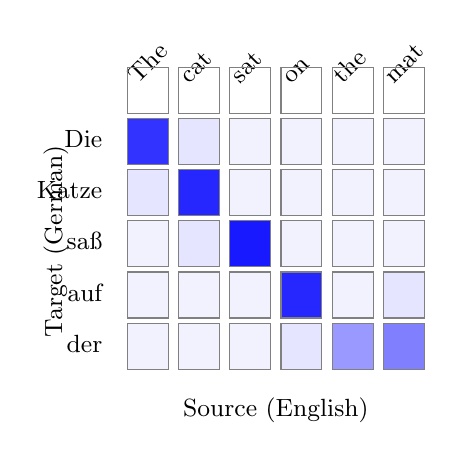
\begin{tikzpicture}[scale=0.65]
        % Grid dimensions
        \def\rows{5}
        \def\cols{6}

        % Column labels (source - English)
        \foreach \j/\w in {1/The, 2/cat, 3/sat, 4/on, 5/the, 6/mat} {
            \node[font=\small, rotate=45, anchor=south west] at (\j-0.2, \rows + 0.3) {\w};
        }

        % Row labels (target - German)
        \foreach \i/\w in {1/Die, 2/Katze, 3/sa\ss{}, 4/auf, 5/der} {
            \node[font=\small, anchor=east] at (0.3, \rows - \i + 0.5) {\w};
        }

        % Attention weights (designed to show alignment patterns)
        % Die -> The (strong)
        \fill[blue!80!white] (1-0.4, 4) rectangle (1+0.4, 4.9);
        \fill[blue!10!white] (2-0.4, 4) rectangle (2+0.4, 4.9);
        \fill[blue!5!white] (3-0.4, 4) rectangle (3+0.4, 4.9);
        \fill[blue!5!white] (4-0.4, 4) rectangle (4+0.4, 4.9);
        \fill[blue!5!white] (5-0.4, 4) rectangle (5+0.4, 4.9);
        \fill[blue!5!white] (6-0.4, 4) rectangle (6+0.4, 4.9);

        % Katze -> cat (strong)
        \fill[blue!10!white] (1-0.4, 3) rectangle (1+0.4, 3.9);
        \fill[blue!85!white] (2-0.4, 3) rectangle (2+0.4, 3.9);
        \fill[blue!5!white] (3-0.4, 3) rectangle (3+0.4, 3.9);
        \fill[blue!5!white] (4-0.4, 3) rectangle (4+0.4, 3.9);
        \fill[blue!5!white] (5-0.4, 3) rectangle (5+0.4, 3.9);
        \fill[blue!5!white] (6-0.4, 3) rectangle (6+0.4, 3.9);

        % saß -> sat (strong)
        \fill[blue!5!white] (1-0.4, 2) rectangle (1+0.4, 2.9);
        \fill[blue!10!white] (2-0.4, 2) rectangle (2+0.4, 2.9);
        \fill[blue!90!white] (3-0.4, 2) rectangle (3+0.4, 2.9);
        \fill[blue!5!white] (4-0.4, 2) rectangle (4+0.4, 2.9);
        \fill[blue!5!white] (5-0.4, 2) rectangle (5+0.4, 2.9);
        \fill[blue!5!white] (6-0.4, 2) rectangle (6+0.4, 2.9);

        % auf -> on (strong)
        \fill[blue!5!white] (1-0.4, 1) rectangle (1+0.4, 1.9);
        \fill[blue!5!white] (2-0.4, 1) rectangle (2+0.4, 1.9);
        \fill[blue!5!white] (3-0.4, 1) rectangle (3+0.4, 1.9);
        \fill[blue!85!white] (4-0.4, 1) rectangle (4+0.4, 1.9);
        \fill[blue!5!white] (5-0.4, 1) rectangle (5+0.4, 1.9);
        \fill[blue!10!white] (6-0.4, 1) rectangle (6+0.4, 1.9);

        % der -> the mat (split attention)
        \fill[blue!5!white] (1-0.4, 0) rectangle (1+0.4, 0.9);
        \fill[blue!5!white] (2-0.4, 0) rectangle (2+0.4, 0.9);
        \fill[blue!5!white] (3-0.4, 0) rectangle (3+0.4, 0.9);
        \fill[blue!10!white] (4-0.4, 0) rectangle (4+0.4, 0.9);
        \fill[blue!40!white] (5-0.4, 0) rectangle (5+0.4, 0.9);
        \fill[blue!50!white] (6-0.4, 0) rectangle (6+0.4, 0.9);

        % Draw grid lines
        \foreach \i in {0, 1, 2, 3, 4, 5} {
            \foreach \j in {1, 2, 3, 4, 5, 6} {
                \draw[gray] (\j-0.4, \i) rectangle (\j+0.4, \i+0.9);
            }
        }

        % Axis labels
        \node at (3.5, -0.8) {\small Source (English)};
        \node[rotate=90] at (-0.8, 2.5) {\small Target (German)};
    \end{tikzpicture}
    \caption{Attention weight visualisation for English-German translation. Each row shows the attention distribution when generating one German word. The roughly diagonal pattern reflects similar word order, with ``der'' (the, dative) attending to both ``the'' and ``mat'' since German articles depend on the noun they modify.}
    \label{fig:bahdanau-alignment}
\end{figure}

\subsection{Bahdanau Attention in the Query-Key-Value Framework}

We can understand Bahdanau attention through the Q/K/V lens introduced in Section~\ref{subsec:qkv}:

\begin{quickref}[Bahdanau Attention as Q/K/V]
\textbf{Query:} The previous decoder hidden state $\mathbf{s}_{t'-1}$

This represents ``what the decoder is looking for''-given what it has generated so far, what source information does it need next?

\textbf{Keys:} The encoder hidden states $\mathbf{h}_1, \ldots, \mathbf{h}_T$

These are the ``addresses'' or ``identifiers'' for each source position. The additive attention function compares the query to each key.

\textbf{Values:} Also the encoder hidden states $\mathbf{h}_1, \ldots, \mathbf{h}_T$

These are the actual information content retrieved. In Bahdanau attention, keys and values are identical.

\textbf{Output:} The context vector $\mathbf{c}_{t'} = \sum_t \alpha_{t't} \mathbf{h}_t$

A weighted combination of values (encoder states), with weights determined by query-key compatibility.
\end{quickref}

This framing reveals a key design choice: in Bahdanau attention, keys and values are the same. Later architectures (including Transformers) will separate them, allowing the model to learn different representations for ``what makes a position findable'' versus ``what information a position provides.''

\subsection{Implementation Considerations}

\begin{quickref}[Practical Implementation of Bahdanau Attention]
\textbf{Efficient batched computation:}

For a batch of $B$ sequences with encoder length $T$ and decoder length $T'$:
\begin{enumerate}
    \item Pre-compute $\mathbf{W}_h \mathbf{H}$ for all encoder states (done once per batch)
    \item At each decoder step, compute $\mathbf{W}_s \mathbf{s}_{t'-1}$ and broadcast-add
    \item Apply $\tanh$ and compute scores with $\mathbf{v}$
    \item Softmax over source dimension (masking padding positions)
    \item Weighted sum over encoder states
\end{enumerate}

\textbf{Masking for variable-length sequences:}

When source sequences have different lengths in a batch, set attention scores to $-\infty$ for padding positions before softmax. This ensures $\alpha_{t't} = 0$ for padded positions.

\textbf{Coverage mechanisms (optional):}

Track cumulative attention to encourage coverage of all source words and discourage repeated attention to the same position. Useful for summarisation and other tasks where under/over-translation is problematic.
\end{quickref}

%==============================================================================
\section{Multi-Head Attention}
\label{sec:multihead}
%==============================================================================

Bahdanau attention computes a single attention distribution over source positions. But there is no reason to limit ourselves to one ``type'' of attention. When reading a sentence, we might simultaneously attend to:
\begin{itemize}
    \item The syntactic head of a phrase
    \item Semantically related words
    \item Positionally adjacent words
    \item Words that resolve ambiguity
\end{itemize}

\textbf{Multi-head attention} addresses this by running multiple attention operations in parallel, each with its own learned parameters. The outputs are then combined, allowing the model to capture diverse relationship types simultaneously.

\subsection{Motivation: Diverse Attention Patterns}

Consider the sentence ``The animal didn't cross the street because it was too tired.'' To understand this sentence fully, a model needs to track multiple types of relationships:

\begin{itemize}
    \item \textbf{Coreference:} ``it'' refers to ``animal'' (requires understanding animacy and context)
    \item \textbf{Causation:} ``because'' links the two clauses
    \item \textbf{Negation scope:} ``didn't'' negates ``cross''
    \item \textbf{Modification:} ``too'' intensifies ``tired''
\end{itemize}

A single attention head might learn one of these patterns well, but would struggle to capture all simultaneously. Multiple heads can specialise in different aspects of the input.

\begin{rigour}[Multi-Head Attention]
\textbf{Idea:} Instead of performing a single attention function, project Q, K, V into multiple subspaces and perform attention in parallel.

\textbf{Input:} Queries $\mathbf{Q} \in \mathbb{R}^{n_q \times d_{\text{model}}}$, Keys $\mathbf{K} \in \mathbb{R}^{n_k \times d_{\text{model}}}$, Values $\mathbf{V} \in \mathbb{R}^{n_k \times d_{\text{model}}}$

\textbf{Step 1: Project to subspaces.}

For each head $i \in \{1, \ldots, h\}$, apply learned linear projections:
\begin{align*}
    \mathbf{Q}_i &= \mathbf{Q} \mathbf{W}_i^Q \in \mathbb{R}^{n_q \times d_k} \\
    \mathbf{K}_i &= \mathbf{K} \mathbf{W}_i^K \in \mathbb{R}^{n_k \times d_k} \\
    \mathbf{V}_i &= \mathbf{V} \mathbf{W}_i^V \in \mathbb{R}^{n_k \times d_v}
\end{align*}

where:
\begin{itemize}
    \item $\mathbf{W}_i^Q \in \mathbb{R}^{d_{\text{model}} \times d_k}$
    \item $\mathbf{W}_i^K \in \mathbb{R}^{d_{\text{model}} \times d_k}$
    \item $\mathbf{W}_i^V \in \mathbb{R}^{d_{\text{model}} \times d_v}$
\end{itemize}

\textbf{Step 2: Compute attention for each head.}

Apply scaled dot-product attention in each subspace:
\[
\text{head}_i = \text{Attention}(\mathbf{Q}_i, \mathbf{K}_i, \mathbf{V}_i) = \text{softmax}\left(\frac{\mathbf{Q}_i \mathbf{K}_i^\top}{\sqrt{d_k}}\right) \mathbf{V}_i
\]

Each head output has shape $\mathbb{R}^{n_q \times d_v}$.

\textbf{Step 3: Concatenate and project.}

Concatenate all head outputs and apply a final linear projection:
\[
\text{MultiHead}(\mathbf{Q}, \mathbf{K}, \mathbf{V}) = \text{Concat}(\text{head}_1, \text{head}_2, \ldots, \text{head}_h) \mathbf{W}^O
\]

where $\mathbf{W}^O \in \mathbb{R}^{(h \cdot d_v) \times d_{\text{model}}}$ projects back to the model dimension.

\textbf{Output shape:} $\mathbb{R}^{n_q \times d_{\text{model}}}$-same as if we had used single-head attention with dimension $d_{\text{model}}$.
\end{rigour}

\begin{figure}[H]
    \centering
    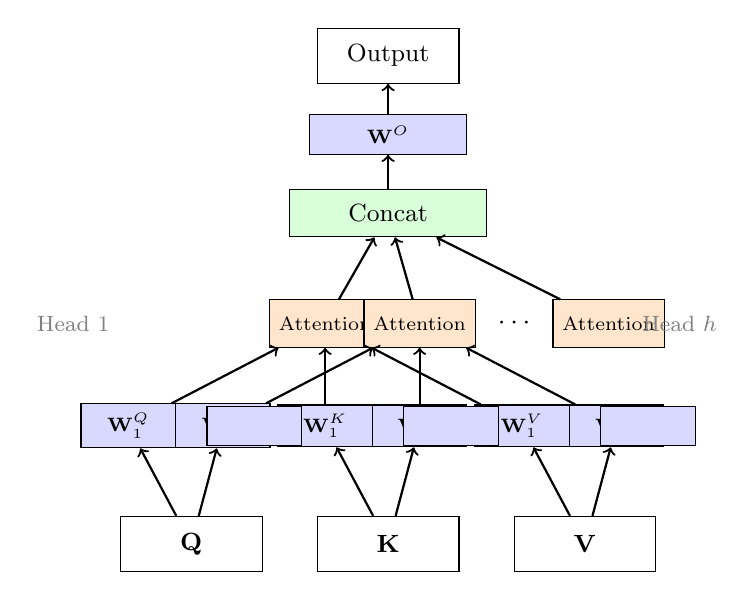
\begin{tikzpicture}[
        box/.style={rectangle, draw, minimum width=1.8cm, minimum height=0.7cm, align=center, font=\small},
        proj/.style={rectangle, draw, fill=blue!15, minimum width=1.2cm, minimum height=0.5cm, align=center, font=\scriptsize},
        attn/.style={rectangle, draw, fill=orange!20, minimum width=1.4cm, minimum height=0.6cm, align=center, font=\scriptsize},
        concat/.style={rectangle, draw, fill=green!15, minimum width=2.5cm, minimum height=0.6cm, align=center, font=\small},
        arrow/.style={->, thick}
    ]
        % Input
        \node[box] (Q) at (0, 0) {$\mathbf{Q}$};
        \node[box] (K) at (2.5, 0) {$\mathbf{K}$};
        \node[box] (V) at (5, 0) {$\mathbf{V}$};

        % Head 1
        \node[proj] (q1) at (-0.8, 1.5) {$\mathbf{W}_1^Q$};
        \node[proj] (k1) at (1.7, 1.5) {$\mathbf{W}_1^K$};
        \node[proj] (v1) at (4.2, 1.5) {$\mathbf{W}_1^V$};
        \node[attn] (a1) at (1.7, 2.8) {Attention};

        % Head 2
        \node[proj] (q2) at (0.4, 1.5) {$\mathbf{W}_2^Q$};
        \node[proj] (k2) at (2.9, 1.5) {$\mathbf{W}_2^K$};
        \node[proj] (v2) at (5.4, 1.5) {$\mathbf{W}_2^V$};
        \node[attn] (a2) at (2.9, 2.8) {Attention};

        % Dots for more heads
        \node at (4.1, 2.8) {$\cdots$};

        % Head h
        \node[proj] (qh) at (0.8, 1.5) {};
        \node[proj] (kh) at (3.3, 1.5) {};
        \node[proj] (vh) at (5.8, 1.5) {};
        \node[attn] (ah) at (5.3, 2.8) {Attention};

        % Arrows to projections
        \draw[arrow] (Q) -- (q1);
        \draw[arrow] (Q) -- (q2);
        \draw[arrow] (K) -- (k1);
        \draw[arrow] (K) -- (k2);
        \draw[arrow] (V) -- (v1);
        \draw[arrow] (V) -- (v2);

        % Arrows to attention
        \draw[arrow] (q1) -- (a1);
        \draw[arrow] (k1) -- (a1);
        \draw[arrow] (v1) -- (a1);
        \draw[arrow] (q2) -- (a2);
        \draw[arrow] (k2) -- (a2);
        \draw[arrow] (v2) -- (a2);

        % Concat
        \node[concat] (concat) at (2.5, 4.2) {Concat};
        \draw[arrow] (a1) -- (concat);
        \draw[arrow] (a2) -- (concat);
        \draw[arrow] (ah) -- (concat);

        % Output projection
        \node[proj, minimum width=2cm] (wo) at (2.5, 5.2) {$\mathbf{W}^O$};
        \draw[arrow] (concat) -- (wo);

        % Output
        \node[box] (out) at (2.5, 6.2) {Output};
        \draw[arrow] (wo) -- (out);

        % Labels
        \node[font=\footnotesize, gray] at (-1.5, 2.8) {Head 1};
        \node[font=\footnotesize, gray] at (6.2, 2.8) {Head $h$};
    \end{tikzpicture}
    \caption{Multi-head attention architecture. Queries, keys, and values are each projected through $h$ different learned projections. Scaled dot-product attention is applied in each subspace independently. The results are concatenated and projected to produce the final output.}
    \label{fig:multihead-attention}
\end{figure}

\subsection{Dimension Management}

A key design choice is how to set the per-head dimensions $d_k$ and $d_v$. The standard approach keeps total computation roughly constant:

\begin{rigour}[Multi-Head Dimension Allocation]
\textbf{Standard configuration:} Set per-head dimensions so that total dimensionality equals the model dimension:
\[
d_k = d_v = \frac{d_{\text{model}}}{h}
\]

\textbf{Example (BERT-Base):}
\begin{itemize}
    \item Model dimension: $d_{\text{model}} = 768$
    \item Number of heads: $h = 12$
    \item Per-head dimension: $d_k = d_v = 768 / 12 = 64$
\end{itemize}

\textbf{Computational cost:} With this configuration, multi-head attention has approximately the same computational cost as single-head attention with full dimension:
\begin{itemize}
    \item Single head at dimension $d$: Attention costs $O(n^2 d)$
    \item $h$ heads at dimension $d/h$ each: Attention costs $h \cdot O(n^2 \cdot d/h) = O(n^2 d)$
\end{itemize}

The projection matrices add $O(d^2)$ parameters per layer, but this is typically subdominant to the attention computation for long sequences.

\textbf{Why this works:} Each head operates in a lower-dimensional subspace, reducing its capacity. But with $h$ heads, the model can attend to $h$ different aspects simultaneously. The concatenation and output projection allow information from all heads to be combined.
\end{rigour}

\subsection{What Do Different Heads Learn?}

Empirical analysis of trained Transformers reveals that different attention heads do indeed specialise:

\begin{quickref}[Observed Head Specialisations]
Studies of trained BERT and GPT models have found heads that specialise in:

\textbf{Syntactic patterns:}
\begin{itemize}
    \item Subject-verb agreement (attending from verb to subject)
    \item Direct objects (attending from verb to object)
    \item Possessive relationships (attending from possessed to possessor)
    \item Prepositional attachment
\end{itemize}

\textbf{Positional patterns:}
\begin{itemize}
    \item Previous token (bigram-like attention)
    \item Next token (anticipatory attention)
    \item First token / \texttt{[CLS]} token
    \item Separator tokens
\end{itemize}

\textbf{Semantic patterns:}
\begin{itemize}
    \item Coreference (pronouns attending to antecedents)
    \item Entity tracking across sentences
    \item Semantic similarity (synonyms, related concepts)
\end{itemize}

\textbf{Task-specific patterns (after fine-tuning):}
\begin{itemize}
    \item Question words attending to answer-relevant spans
    \item Named entity boundaries
    \item Sentiment-bearing words
\end{itemize}

\textbf{Caveat:} Not all heads are equally interpretable or useful. Some heads appear redundant or encode diffuse patterns. Pruning experiments show that many heads can be removed with minimal performance loss.
\end{quickref}

%==============================================================================
\section{Self-Attention}
\label{sec:self-attention}
%==============================================================================

All the attention mechanisms we have discussed so far involve attention \textit{between} two sequences: the decoder attending to the encoder (Bahdanau), or queries attending to a separate key-value store. \textbf{Self-attention} is the special case where a single sequence attends to itself-every position can attend to every other position (including itself) within the same sequence.

This seemingly simple change has profound implications. Self-attention enables direct interaction between any two positions in a sequence, regardless of their distance. This contrasts sharply with RNNs (where distant positions interact only through a chain of hidden states) and CNNs (where interaction range is limited by kernel size).

\subsection{Definition and Intuition}

\begin{rigour}[Self-Attention]
\textbf{Setup:} Given a sequence of $n$ vectors $\mathbf{x}_1, \mathbf{x}_2, \ldots, \mathbf{x}_n \in \mathbb{R}^d$ (e.g., word embeddings).

\textbf{Self-attention output:} For each position $i$, compute:
\[
\mathbf{y}_i = \sum_{j=1}^{n} \alpha_{ij} \, \mathbf{v}_j
\]

where:
\begin{itemize}
    \item $\alpha_{ij}$ is the attention weight from position $i$ to position $j$
    \item $\mathbf{v}_j$ is the value vector at position $j$
\end{itemize}

\textbf{Key distinction:} In self-attention, queries, keys, and values are all derived from the \textit{same} input sequence. Typically:
\begin{align*}
    \mathbf{q}_i &= \mathbf{x}_i \mathbf{W}^Q \quad \text{(query at position } i \text{)} \\
    \mathbf{k}_j &= \mathbf{x}_j \mathbf{W}^K \quad \text{(key at position } j \text{)} \\
    \mathbf{v}_j &= \mathbf{x}_j \mathbf{W}^V \quad \text{(value at position } j \text{)}
\end{align*}

\textbf{Matrix form:} With $\mathbf{X} \in \mathbb{R}^{n \times d}$ (input), $\mathbf{W}^Q, \mathbf{W}^K \in \mathbb{R}^{d \times d_k}$, $\mathbf{W}^V \in \mathbb{R}^{d \times d_v}$:
\begin{align*}
    \mathbf{Q} &= \mathbf{X} \mathbf{W}^Q \in \mathbb{R}^{n \times d_k} \\
    \mathbf{K} &= \mathbf{X} \mathbf{W}^K \in \mathbb{R}^{n \times d_k} \\
    \mathbf{V} &= \mathbf{X} \mathbf{W}^V \in \mathbb{R}^{n \times d_v}
\end{align*}

\textbf{Scaled dot-product self-attention:}
\[
\text{SelfAttention}(\mathbf{X}) = \text{softmax}\left(\frac{\mathbf{Q} \mathbf{K}^\top}{\sqrt{d_k}}\right) \mathbf{V}
\]

\textbf{Output:} $\mathbf{Y} \in \mathbb{R}^{n \times d_v}$, where each $\mathbf{y}_i$ is a \textit{contextualised} representation of position $i$, incorporating information from all positions weighted by attention.
\end{rigour}

The intuition is that each position ``asks a question'' (via its query) about what information it needs, ``broadcasts its identity'' (via its key) so others can find it, and ``provides its content'' (via its value) to positions that attend to it.

\begin{rigour}[Self-Attention: Worked Example]
Consider the sentence ``The cat sat'' with three token positions.

\textbf{Input embeddings} (simplified 4-dimensional):
\begin{align*}
    \mathbf{x}_1 &= [0.2, 0.1, 0.8, 0.3]^\top \quad \text{(``The'')} \\
    \mathbf{x}_2 &= [0.9, 0.7, 0.2, 0.1]^\top \quad \text{(``cat'')} \\
    \mathbf{x}_3 &= [0.3, 0.8, 0.5, 0.9]^\top \quad \text{(``sat'')}
\end{align*}

\textbf{Simplified scenario:} Assume identity projections ($\mathbf{W}^Q = \mathbf{W}^K = \mathbf{W}^V = \mathbf{I}$) so $\mathbf{q}_i = \mathbf{k}_i = \mathbf{v}_i = \mathbf{x}_i$.

\textbf{Step 1: Compute attention scores.}

The score from position $i$ to position $j$ is $\mathbf{q}_i^\top \mathbf{k}_j$:
\[
\mathbf{Q} \mathbf{K}^\top = \begin{bmatrix}
    \mathbf{x}_1^\top \mathbf{x}_1 & \mathbf{x}_1^\top \mathbf{x}_2 & \mathbf{x}_1^\top \mathbf{x}_3 \\
    \mathbf{x}_2^\top \mathbf{x}_1 & \mathbf{x}_2^\top \mathbf{x}_2 & \mathbf{x}_2^\top \mathbf{x}_3 \\
    \mathbf{x}_3^\top \mathbf{x}_1 & \mathbf{x}_3^\top \mathbf{x}_2 & \mathbf{x}_3^\top \mathbf{x}_3
\end{bmatrix}
\]

Computing the dot products:
\begin{align*}
    \mathbf{x}_1^\top \mathbf{x}_1 &= 0.04 + 0.01 + 0.64 + 0.09 = 0.78 \\
    \mathbf{x}_1^\top \mathbf{x}_2 &= 0.18 + 0.07 + 0.16 + 0.03 = 0.44 \\
    \mathbf{x}_1^\top \mathbf{x}_3 &= 0.06 + 0.08 + 0.40 + 0.27 = 0.81 \\
    &\vdots
\end{align*}

After computing all entries and scaling by $\sqrt{4} = 2$:
\[
\frac{\mathbf{Q} \mathbf{K}^\top}{\sqrt{d}} \approx \begin{bmatrix}
    0.39 & 0.22 & 0.41 \\
    0.22 & 0.68 & 0.54 \\
    0.41 & 0.54 & 0.90
\end{bmatrix}
\]

\textbf{Step 2: Apply softmax row-wise.}

Each row becomes a probability distribution:
\[
\boldsymbol{\alpha} = \text{softmax}\left(\frac{\mathbf{Q} \mathbf{K}^\top}{\sqrt{d}}\right) \approx \begin{bmatrix}
    0.33 & 0.28 & 0.39 \\
    0.26 & 0.41 & 0.33 \\
    0.27 & 0.31 & 0.42
\end{bmatrix}
\]

\textbf{Step 3: Compute outputs.}

For position 1 (``The''):
\[
\mathbf{y}_1 = 0.33 \cdot \mathbf{x}_1 + 0.28 \cdot \mathbf{x}_2 + 0.39 \cdot \mathbf{x}_3
\]

This output is a weighted combination of all three word embeddings, with weights learned based on their relevance to position 1.

\textbf{Interpretation:} The output $\mathbf{y}_1$ is no longer just ``The''-it is a \textit{contextualised} representation that incorporates information from ``cat'' and ``sat''. After self-attention, every position ``knows about'' every other position.
\end{rigour}

\subsection{Properties of Self-Attention}

Self-attention has several distinctive properties that make it powerful for sequence modelling:

\begin{quickref}[Self-Attention: Key Properties]
\textbf{1. Constant path length.}

Any two positions interact directly in a single self-attention layer. The maximum path length for information to travel is $O(1)$.

Compare with:
\begin{itemize}
    \item RNNs: $O(n)$ steps for position 1 to influence position $n$
    \item CNNs: $O(\log_k n)$ layers for receptive field to cover full sequence
\end{itemize}

This short path length facilitates learning long-range dependencies and provides stable gradients.

\textbf{2. Full parallelisation.}

All positions can be computed simultaneously-no sequential dependency between positions within a layer. This contrasts with RNNs, where position $t$ depends on position $t-1$.

\textbf{3. Global context.}

Each output position has access to the entire input sequence. There is no locality bias as in CNNs.

\textbf{4. Permutation equivariance.}

If we permute the input sequence, the output is permuted identically (with correspondingly permuted attention weights). Self-attention has no inherent notion of position-this must be added via positional encoding.
\end{quickref}

\begin{rigour}[Complexity Analysis: Self-Attention vs RNN vs CNN]
For a sequence of length $n$ with model dimension $d$:

\begin{center}
\begin{tabular}{lccc}
\toprule
\textbf{Property} & \textbf{Self-Attention} & \textbf{RNN} & \textbf{CNN} \\
\midrule
Computation per layer & $O(n^2 \cdot d)$ & $O(n \cdot d^2)$ & $O(k \cdot n \cdot d^2)$ \\
Sequential operations & $O(1)$ & $O(n)$ & $O(1)$ \\
Maximum path length & $O(1)$ & $O(n)$ & $O(\log_k n)$ \\
Memory per layer & $O(n^2 + n \cdot d)$ & $O(n \cdot d)$ & $O(n \cdot d)$ \\
\bottomrule
\end{tabular}
\end{center}

\textbf{Analysis:}
\begin{itemize}
    \item \textbf{When $n < d$:} Self-attention is faster than RNNs
    \item \textbf{When $n > d$:} Self-attention becomes the bottleneck (quadratic in $n$)
    \item \textbf{For parallelisation:} Self-attention and CNNs are fully parallel; RNNs are sequential
    \item \textbf{For long-range dependencies:} Self-attention has the shortest path
\end{itemize}

\textbf{Practical implications:} Self-attention excels for moderate sequence lengths (up to a few thousand tokens) on modern GPUs. For very long sequences (10,000+), efficient attention variants become necessary.
\end{rigour}

\begin{redbox}
\textbf{The Quadratic Complexity Bottleneck}

Self-attention computes pairwise interactions between all positions, giving $O(n^2)$ complexity:

\textbf{Concrete numbers:}
\begin{itemize}
    \item $n = 512$ tokens: $\sim$262,000 attention scores per head
    \item $n = 2048$ tokens: $\sim$4.2 million attention scores per head
    \item $n = 8192$ tokens: $\sim$67 million attention scores per head
\end{itemize}

With 12 layers and 12 heads, a single forward pass on 8192 tokens computes nearly 10 billion attention scores!

\textbf{Memory is often the binding constraint:} The attention matrix must be stored for backpropagation. For $n = 8192$ with 16-bit precision, each attention matrix requires $\sim$134 MB per head per layer.

\textbf{Mitigations:}
\begin{itemize}
    \item \textbf{Flash Attention:} Memory-efficient implementation that avoids materialising the full attention matrix; uses tiling and recomputation.
    \item \textbf{Sparse attention:} Attend only to a subset of positions (local windows, strided patterns, learned sparsity).
    \item \textbf{Linear attention:} Approximate softmax attention with $O(n)$ complexity using kernel methods.
    \item \textbf{Sliding window attention:} Each position attends only to a local window, with global tokens for long-range.
\end{itemize}

These are active research areas, with new efficient attention methods appearing regularly.
\end{redbox}

\subsection{Masked Self-Attention for Autoregressive Generation}

For autoregressive models (like GPT), we need to prevent positions from attending to future positions. This is achieved through \textbf{causal masking}.

\begin{rigour}[Causal (Masked) Self-Attention]
\textbf{Problem:} During training, the full target sequence is available. Without masking, position $t$ could ``cheat'' by looking at positions $t+1, t+2, \ldots$

\textbf{Solution:} Apply a mask that prevents attention to future positions:
\[
\text{Mask}_{ij} = \begin{cases}
    0 & \text{if } j \leq i \quad \text{(can attend)} \\
    -\infty & \text{if } j > i \quad \text{(cannot attend)}
\end{cases}
\]

\textbf{Masked attention computation:}
\[
\text{MaskedAttention}(\mathbf{Q}, \mathbf{K}, \mathbf{V}) = \text{softmax}\left(\frac{\mathbf{Q} \mathbf{K}^\top + \text{Mask}}{\sqrt{d_k}}\right) \mathbf{V}
\]

Adding $-\infty$ before softmax ensures those positions get zero attention weight:
\[
\text{softmax}(\ldots, -\infty, \ldots)_i = \frac{e^{-\infty}}{\ldots} = 0
\]

\textbf{Resulting attention pattern:} Lower triangular-position $i$ can only attend to positions $\{1, 2, \ldots, i\}$.

\textbf{During inference:} Masking is naturally satisfied since future tokens have not been generated yet.
\end{rigour}

%==============================================================================
\section{Positional Encoding}
\label{sec:positional-encoding}
%==============================================================================

We noted that self-attention is \textbf{permutation equivariant}-if we shuffle the input tokens, the output is shuffled identically. But word order matters crucially in language: ``dog bites man'' means something very different from ``man bites dog.'' Without position information, a self-attention layer cannot distinguish these sentences!

\textbf{Positional encoding} injects position information into the input representations, breaking the permutation equivariance and allowing the model to learn position-dependent patterns.

\subsection{The Problem: Order Blindness}

\begin{rigour}[Permutation Equivariance of Self-Attention]
\textbf{Claim:} Self-attention (without positional encoding) is permutation equivariant.

\textbf{Formal statement:} Let $\pi$ be a permutation of $\{1, \ldots, n\}$, and let $\mathbf{P}_\pi$ be the corresponding permutation matrix. Then:
\[
\text{SelfAttention}(\mathbf{P}_\pi \mathbf{X}) = \mathbf{P}_\pi \, \text{SelfAttention}(\mathbf{X})
\]

\textbf{Proof sketch:}
\begin{enumerate}
    \item Permuting $\mathbf{X}$ permutes $\mathbf{Q}$, $\mathbf{K}$, $\mathbf{V}$ identically (since they are linear transformations of $\mathbf{X}$).
    \item The attention scores $\mathbf{Q} \mathbf{K}^\top$ are permuted: rows by $\pi$ (from $\mathbf{Q}$), columns by $\pi$ (from $\mathbf{K}$).
    \item Softmax is applied row-wise, so row permutation is preserved.
    \item Multiplying by permuted $\mathbf{V}$ gives output permuted by $\pi$.
\end{enumerate}

\textbf{Implication:} The \textit{content} of each output depends only on the \textit{set} of inputs, not their order. ``The cat sat'' and ``sat cat The'' would produce the same outputs (up to permutation).

\textbf{This is unacceptable for language:} Position carries meaning. We need to explicitly encode position.
\end{rigour}

\subsection{Sinusoidal Positional Encoding}

The original Transformer paper introduced fixed sinusoidal positional encodings. The idea is to add position-specific vectors to the input embeddings.

\begin{rigour}[Sinusoidal Positional Encoding]
\textbf{Method:} Add a position-dependent vector to each token embedding:
\[
\tilde{\mathbf{x}}_i = \mathbf{x}_i + \mathbf{p}_i
\]
where $\mathbf{p}_i \in \mathbb{R}^d$ encodes position $i$.

\textbf{Sinusoidal formula:} For position $\text{pos}$ and dimension $i$:
\begin{align*}
    \text{PE}(\text{pos}, 2i) &= \sin\left(\frac{\text{pos}}{10000^{2i/d}}\right) \\
    \text{PE}(\text{pos}, 2i+1) &= \cos\left(\frac{\text{pos}}{10000^{2i/d}}\right)
\end{align*}

\textbf{Interpretation:}
\begin{itemize}
    \item Each dimension $i$ corresponds to a sinusoid with a different frequency
    \item Low dimensions (small $i$): Low frequency, slow variation with position
    \item High dimensions (large $i$): High frequency, rapid variation with position
    \item The position is encoded across all dimensions, like a binary representation but with sinusoids
\end{itemize}

\textbf{Why sinusoids?}

\textbf{1. Unique encoding:} Each position has a distinct encoding vector.

\textbf{2. Bounded values:} All values are in $[-1, 1]$, compatible with normalised embeddings.

\textbf{3. Relative position via linear transformation:} For any fixed offset $k$:
\[
\text{PE}(\text{pos} + k) = f_k(\text{PE}(\text{pos}))
\]
where $f_k$ is a linear transformation. This allows the model to learn relative position patterns.

\textbf{Proof of linear transformation property:}

Using trigonometric identities:
\begin{align*}
    \sin(\omega(\text{pos} + k)) &= \sin(\omega \cdot \text{pos}) \cos(\omega k) + \cos(\omega \cdot \text{pos}) \sin(\omega k) \\
    \cos(\omega(\text{pos} + k)) &= \cos(\omega \cdot \text{pos}) \cos(\omega k) - \sin(\omega \cdot \text{pos}) \sin(\omega k)
\end{align*}

This is a linear combination of $\sin(\omega \cdot \text{pos})$ and $\cos(\omega \cdot \text{pos})$ with coefficients depending only on $k$.

\textbf{4. Extrapolation:} Can encode positions beyond those seen during training (unlike learned embeddings).
\end{rigour}

\begin{figure}[H]
    \centering
    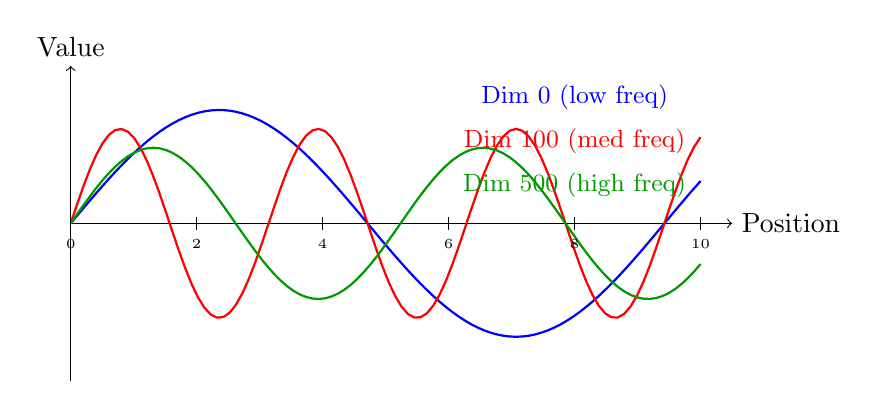
\begin{tikzpicture}[scale=0.8]
        % Axes
        \draw[->] (0, 0) -- (10.5, 0) node[right] {Position};
        \draw[->] (0, -2.5) -- (0, 2.5) node[above] {Value};

        % Different frequencies
        \draw[blue, thick, domain=0:10, samples=100] plot (\x, {1.8*sin(deg(\x/1.5))});
        \draw[red, thick, domain=0:10, samples=100] plot (\x, {1.5*sin(deg(\x/0.5))});
        \draw[green!60!black, thick, domain=0:10, samples=100] plot (\x, {1.2*sin(deg(\x*1.2))});

        % Legend
        \node[blue] at (8, 2) {\small Dim 0 (low freq)};
        \node[red] at (8, 1.3) {\small Dim 100 (med freq)};
        \node[green!60!black] at (8, 0.6) {\small Dim 500 (high freq)};

        % Position markers
        \foreach \x in {0, 2, 4, 6, 8, 10} {
            \draw (\x, 0.1) -- (\x, -0.1) node[below] {\tiny \x};
        }
    \end{tikzpicture}
    \caption{Sinusoidal positional encoding at different dimensions. Lower dimensions vary slowly with position (low frequency); higher dimensions vary rapidly (high frequency). The combination of frequencies at all dimensions provides a unique ``signature'' for each position.}
    \label{fig:sinusoidal-encoding}
\end{figure}

\subsection{Alternative Positional Encoding Methods}

\begin{quickref}[Positional Encoding Variants]
\textbf{1. Learned positional embeddings:}
\begin{itemize}
    \item Train a separate embedding $\mathbf{p}_i$ for each position $i \in \{1, \ldots, L_{\max}\}$
    \item More flexible than sinusoidal-can learn arbitrary position-specific patterns
    \item Cannot extrapolate to positions beyond $L_{\max}$
    \item Used in BERT, GPT-2, and most modern models
\end{itemize}

\textbf{2. Relative positional encoding:}
\begin{itemize}
    \item Encode the \textit{relative distance} between positions rather than absolute position
    \item More natural for many tasks (``the word 3 positions ago'' vs ``position 47'')
    \item Attention score includes a learned bias depending on $i - j$
    \item Used in Transformer-XL, T5
\end{itemize}

\textbf{3. Rotary Position Embedding (RoPE):}
\begin{itemize}
    \item Encode position by \textit{rotating} query and key vectors in embedding space
    \item Rotation angle depends on position
    \item Dot product between rotated vectors depends on relative position
    \item Combines benefits of absolute and relative encoding
    \item Used in LLaMA, GPT-NeoX, and many recent LLMs
\end{itemize}

\textbf{4. ALiBi (Attention with Linear Biases):}
\begin{itemize}
    \item Add a linear penalty to attention scores based on distance: $\text{score}_{ij} \mapsto \text{score}_{ij} - m \cdot |i - j|$
    \item No learned position parameters
    \item Excellent extrapolation to longer sequences
    \item Used in BLOOM
\end{itemize}
\end{quickref}

%==============================================================================
\section{The Transformer Architecture}
\label{sec:transformer}
%==============================================================================

We now have all the building blocks: scaled dot-product attention, multi-head attention, self-attention, and positional encoding. The \textbf{Transformer} architecture, introduced in the landmark paper ``Attention Is All You Need'' (Vaswani et al., 2017), combines these components into a complete model for sequence-to-sequence learning-without any recurrence or convolution.

The title of the paper was not hyperbole. Transformers have since become the dominant architecture across virtually all of deep learning: language models (GPT, BERT, LLaMA), vision models (ViT, DINO), speech models (Whisper), multimodal models (CLIP, Flamingo), and even reinforcement learning (Decision Transformer).

\begin{quickref}[Transformer: Historical Impact]
\textbf{The paper:} ``Attention Is All You Need'' (Vaswani et al., NeurIPS 2017)

\textbf{Key claim:} A model based \textit{entirely} on attention (no RNNs, no CNNs) can achieve state-of-the-art results on machine translation while being more parallelisable and faster to train.

\textbf{Results on WMT 2014 English-German translation:}
\begin{itemize}
    \item Transformer: 28.4 BLEU (new state-of-the-art)
    \item Previous best: 26.4 BLEU (ensemble of models)
    \item Training time: 3.5 days on 8 GPUs (vs weeks for RNN models)
\end{itemize}

\textbf{Subsequent impact:}
\begin{itemize}
    \item BERT (2018): Transformer encoder for NLP understanding
    \item GPT (2018): Transformer decoder for text generation
    \item ViT (2020): Transformer for computer vision
    \item GPT-3 (2020): 175B parameter language model
    \item ChatGPT (2022): Conversational AI based on Transformers
\end{itemize}
\end{quickref}

\subsection{The Transformer Encoder}

The encoder transforms an input sequence into a sequence of contextualised representations. It consists of a stack of identical layers, each containing two sub-layers.

\begin{rigour}[Transformer Encoder Layer]
Each encoder layer consists of:

\textbf{Sub-layer 1: Multi-Head Self-Attention}
\[
\mathbf{Z}_{\text{attn}} = \text{MultiHead}(\mathbf{X}, \mathbf{X}, \mathbf{X})
\]

All three inputs (Q, K, V) come from the same source: the layer input $\mathbf{X}$.

\textbf{Sub-layer 2: Position-wise Feed-Forward Network (FFN)}
\[
\text{FFN}(\mathbf{z}) = \text{ReLU}(\mathbf{z} \mathbf{W}_1 + \mathbf{b}_1) \mathbf{W}_2 + \mathbf{b}_2
\]

Applied independently to each position (same parameters for all positions).

Typically: $\mathbf{W}_1 \in \mathbb{R}^{d_{\text{model}} \times d_{\text{ff}}}$, $\mathbf{W}_2 \in \mathbb{R}^{d_{\text{ff}} \times d_{\text{model}}}$ with $d_{\text{ff}} = 4 \cdot d_{\text{model}}$.

\textbf{Residual connections:} Each sub-layer has a residual connection around it.

\textbf{Layer normalisation:} Applied after each residual connection.

\textbf{Full encoder layer:}
\begin{align*}
    \mathbf{Z}_1 &= \text{LayerNorm}(\mathbf{X} + \text{MultiHead}(\mathbf{X}, \mathbf{X}, \mathbf{X})) \\
    \mathbf{Z}_2 &= \text{LayerNorm}(\mathbf{Z}_1 + \text{FFN}(\mathbf{Z}_1))
\end{align*}

Output $\mathbf{Z}_2$ becomes input to the next encoder layer.

\textbf{Full encoder:} Stack $N$ identical layers (typically $N = 6$ or $N = 12$).
\end{rigour}

\begin{figure}[H]
    \centering
    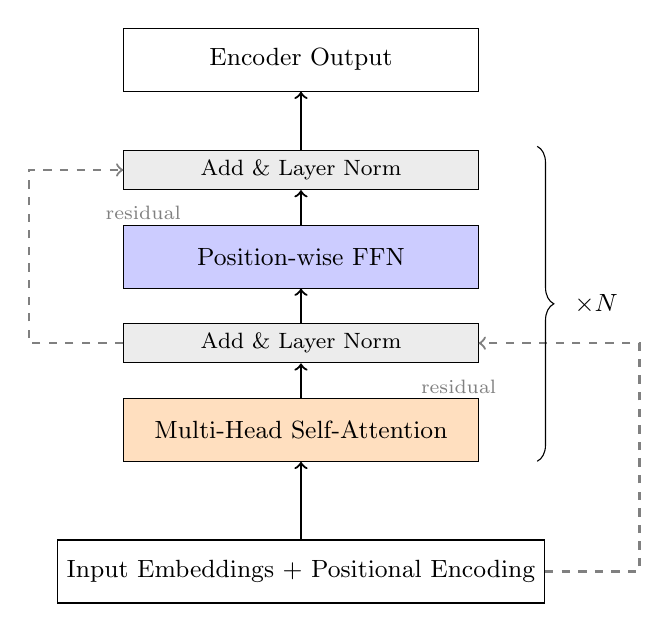
\begin{tikzpicture}[
        block/.style={rectangle, draw, minimum width=4.5cm, minimum height=0.8cm, align=center, font=\small},
        attn/.style={rectangle, draw, fill=orange!25, minimum width=4.5cm, minimum height=0.8cm, align=center, font=\small},
        ffn/.style={rectangle, draw, fill=blue!20, minimum width=4.5cm, minimum height=0.8cm, align=center, font=\small},
        norm/.style={rectangle, draw, fill=gray!15, minimum width=4.5cm, minimum height=0.5cm, align=center, font=\footnotesize},
        arrow/.style={->, thick}
    ]
        % Input
        \node[block] (input) at (0, 0) {Input Embeddings + Positional Encoding};

        % Encoder layer
        \node[attn] (attn) at (0, 1.8) {Multi-Head Self-Attention};
        \node[norm] (norm1) at (0, 2.9) {Add \& Layer Norm};
        \node[ffn] (ffn) at (0, 4) {Position-wise FFN};
        \node[norm] (norm2) at (0, 5.1) {Add \& Layer Norm};

        % Main flow
        \draw[arrow] (input) -- (attn);
        \draw[arrow] (attn) -- (norm1);
        \draw[arrow] (norm1) -- (ffn);
        \draw[arrow] (ffn) -- (norm2);

        % Residual connections
        \draw[arrow, dashed, gray] (input.east) -- ++(1.2, 0) |- (norm1.east);
        \draw[arrow, dashed, gray] (norm1.west) -- ++(-1.2, 0) |- (norm2.west);

        % N times bracket
        \draw[decorate, decoration={brace, amplitude=6pt, mirror}]
            (3, 1.4) -- (3, 5.4) node[midway, right=10pt, font=\small] {$\times N$};

        % Output
        \node[block] (output) at (0, 6.5) {Encoder Output};
        \draw[arrow] (norm2) -- (output);

        % Annotation
        \node[font=\scriptsize, gray, right] at (1.4, 2.35) {residual};
        \node[font=\scriptsize, gray, left] at (-1.4, 4.55) {residual};
    \end{tikzpicture}
    \caption{Transformer encoder layer. Multi-head self-attention allows each position to attend to all positions. The position-wise FFN adds nonlinearity and capacity. Residual connections and layer normalisation facilitate training of deep stacks. The encoder consists of $N$ identical layers.}
    \label{fig:transformer-encoder}
\end{figure}

\textbf{Why the FFN?} The self-attention layer is essentially a weighted averaging operation-linear in the values. The FFN adds nonlinearity and provides additional model capacity. Empirically, the FFN parameters account for about two-thirds of the model's parameters and are crucial for performance.

\textbf{Why layer normalisation?} Layer normalisation (see Week 5 discussion of batch normalisation) stabilises training by normalising activations. Unlike batch normalisation, it normalises across features rather than across the batch, making it suitable for variable-length sequences and small batches.

\subsection{The Transformer Decoder}

The decoder generates the output sequence autoregressively. It is similar to the encoder but with an additional \textbf{cross-attention} layer that attends to the encoder output.

\begin{rigour}[Transformer Decoder Layer]
Each decoder layer consists of three sub-layers:

\textbf{Sub-layer 1: Masked Multi-Head Self-Attention}
\[
\mathbf{Z}_1 = \text{MaskedMultiHead}(\mathbf{Y}, \mathbf{Y}, \mathbf{Y})
\]

Causal masking prevents attending to future positions (see Section~\ref{sec:self-attention}).

\textbf{Sub-layer 2: Multi-Head Cross-Attention}
\[
\mathbf{Z}_2 = \text{MultiHead}(\mathbf{Z}_1, \mathbf{H}_{\text{enc}}, \mathbf{H}_{\text{enc}})
\]

\begin{itemize}
    \item Queries: from decoder (previous sub-layer output $\mathbf{Z}_1$)
    \item Keys and Values: from encoder output $\mathbf{H}_{\text{enc}}$
\end{itemize}

This allows the decoder to attend to the input sequence-the analogue of Bahdanau attention in the Transformer.

\textbf{Sub-layer 3: Position-wise FFN}

Same as encoder FFN.

\textbf{Full decoder layer:}
\begin{align*}
    \mathbf{Z}_1 &= \text{LayerNorm}(\mathbf{Y} + \text{MaskedMultiHead}(\mathbf{Y}, \mathbf{Y}, \mathbf{Y})) \\
    \mathbf{Z}_2 &= \text{LayerNorm}(\mathbf{Z}_1 + \text{MultiHead}(\mathbf{Z}_1, \mathbf{H}_{\text{enc}}, \mathbf{H}_{\text{enc}})) \\
    \mathbf{Z}_3 &= \text{LayerNorm}(\mathbf{Z}_2 + \text{FFN}(\mathbf{Z}_2))
\end{align*}

Each sub-layer has residual connections and layer normalisation.
\end{rigour}

\begin{figure}[H]
    \centering
    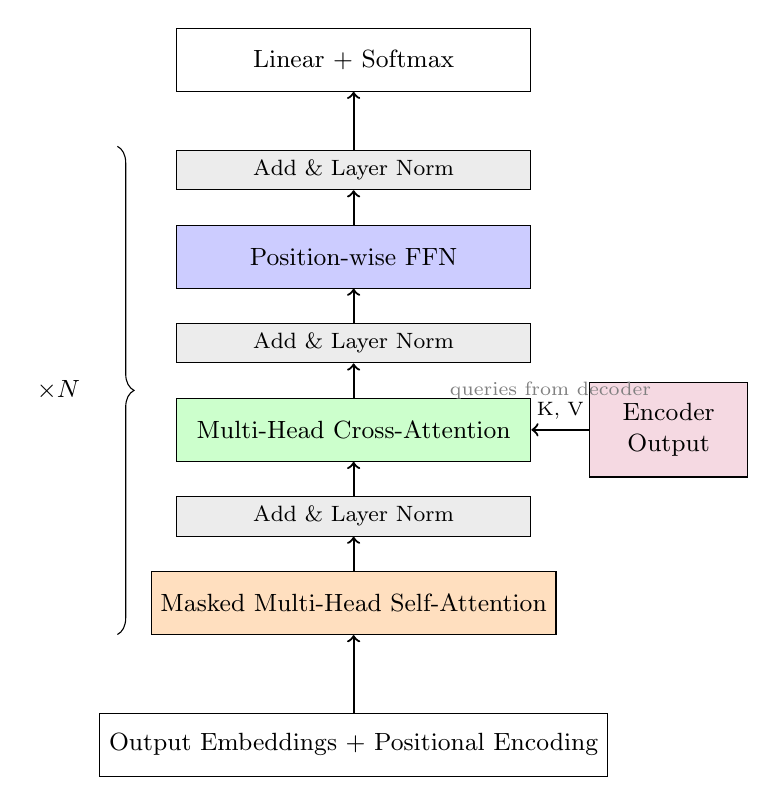
\begin{tikzpicture}[
        block/.style={rectangle, draw, minimum width=4.5cm, minimum height=0.8cm, align=center, font=\small},
        attn/.style={rectangle, draw, fill=orange!25, minimum width=4.5cm, minimum height=0.8cm, align=center, font=\small},
        cross/.style={rectangle, draw, fill=green!20, minimum width=4.5cm, minimum height=0.8cm, align=center, font=\small},
        ffn/.style={rectangle, draw, fill=blue!20, minimum width=4.5cm, minimum height=0.8cm, align=center, font=\small},
        norm/.style={rectangle, draw, fill=gray!15, minimum width=4.5cm, minimum height=0.5cm, align=center, font=\footnotesize},
        enc/.style={rectangle, draw, fill=purple!15, minimum width=2cm, minimum height=1.2cm, align=center, font=\small},
        arrow/.style={->, thick}
    ]
        % Input
        \node[block] (input) at (0, 0) {Output Embeddings + Positional Encoding};

        % Decoder layer
        \node[attn] (attn) at (0, 1.8) {Masked Multi-Head Self-Attention};
        \node[norm] (norm1) at (0, 2.9) {Add \& Layer Norm};
        \node[cross] (cross) at (0, 4) {Multi-Head Cross-Attention};
        \node[norm] (norm2) at (0, 5.1) {Add \& Layer Norm};
        \node[ffn] (ffn) at (0, 6.2) {Position-wise FFN};
        \node[norm] (norm3) at (0, 7.3) {Add \& Layer Norm};

        % Encoder output
        \node[enc] (enc) at (4, 4) {Encoder\\Output};

        % Main flow
        \draw[arrow] (input) -- (attn);
        \draw[arrow] (attn) -- (norm1);
        \draw[arrow] (norm1) -- (cross);
        \draw[arrow] (cross) -- (norm2);
        \draw[arrow] (norm2) -- (ffn);
        \draw[arrow] (ffn) -- (norm3);

        % Cross-attention from encoder
        \draw[arrow] (enc) -- (cross.east) node[midway, above, font=\scriptsize] {K, V};

        % N times bracket
        \draw[decorate, decoration={brace, amplitude=6pt, mirror}]
            (-3, 1.4) -- (-3, 7.6) node[midway, left=10pt, font=\small] {$\times N$};

        % Output
        \node[block] (output) at (0, 8.7) {Linear + Softmax};
        \draw[arrow] (norm3) -- (output);

        % Annotation
        \node[font=\scriptsize, gray] at (2.5, 4.5) {queries from decoder};
    \end{tikzpicture}
    \caption{Transformer decoder layer. Masked self-attention prevents looking at future positions. Cross-attention allows attending to the encoder output (keys and values from encoder, queries from decoder). The final linear layer and softmax produce token probabilities.}
    \label{fig:transformer-decoder}
\end{figure}

\subsection{Transformer Architectural Variants}

The original Transformer used both encoder and decoder for translation. Subsequent work showed that simpler variants are often more effective for specific tasks.

\begin{quickref}[Transformer Architecture Types]
\textbf{1. Encoder-Decoder (Original Transformer, T5, BART):}
\begin{itemize}
    \item Full encoder processes input; full decoder generates output
    \item Cross-attention connects decoder to encoder
    \item \textbf{Best for:} Sequence-to-sequence tasks (translation, summarisation)
    \item \textbf{Examples:} Original Transformer, T5, BART, mBART
\end{itemize}

\textbf{2. Encoder-Only (BERT, RoBERTa):}
\begin{itemize}
    \item Only the encoder stack
    \item Bidirectional self-attention (no causal masking)
    \item Output: Contextualised representations for each input token
    \item \textbf{Best for:} Understanding tasks (classification, NER, extractive QA)
    \item \textbf{Examples:} BERT, RoBERTa, ALBERT, ELECTRA, DeBERTa
\end{itemize}

\textbf{3. Decoder-Only (GPT, LLaMA, Claude):}
\begin{itemize}
    \item Only the decoder stack (with causal masking, no cross-attention)
    \item Unidirectional: each token attends only to previous tokens
    \item \textbf{Best for:} Text generation, language modelling, few-shot learning
    \item \textbf{Examples:} GPT-2, GPT-3, GPT-4, LLaMA, Claude, Mistral
\end{itemize}

\textbf{Why decoder-only dominates modern LLMs:}
\begin{itemize}
    \item Simpler architecture (one stack, no cross-attention)
    \item Natural fit for autoregressive language modelling
    \item Scales more predictably with model size
    \item Easier to train with simple next-token prediction objective
\end{itemize}
\end{quickref}

%==============================================================================
\section{BERT: Bidirectional Encoder Representations}
\label{sec:bert}
%==============================================================================

BERT (Bidirectional Encoder Representations from Transformers), introduced by Devlin et al.\ (2019), demonstrated the power of \textbf{pretraining} Transformer encoders on large text corpora. The key insight was that bidirectional context-attending to both left and right context simultaneously-produces much richer representations than unidirectional models.

BERT's ``pretrain, then fine-tune'' paradigm became the standard approach for NLP: train a large model on massive unlabelled data, then adapt it to specific tasks with relatively little labelled data.

\subsection{Architecture and Pretraining}

\begin{rigour}[BERT Architecture]
\textbf{Model structure:}
\begin{itemize}
    \item Encoder-only Transformer (no decoder)
    \item Bidirectional self-attention: each token attends to all tokens (no causal masking)
\end{itemize}

\textbf{Model sizes:}
\begin{center}
\begin{tabular}{lccccc}
\toprule
\textbf{Model} & \textbf{Layers} & \textbf{Hidden} & \textbf{Heads} & \textbf{FFN} & \textbf{Parameters} \\
\midrule
BERT-Base & 12 & 768 & 12 & 3072 & 110M \\
BERT-Large & 24 & 1024 & 16 & 4096 & 340M \\
\bottomrule
\end{tabular}
\end{center}

\textbf{Input representation:}
\[
\text{Input} = \text{Token Embedding} + \text{Segment Embedding} + \text{Position Embedding}
\]

\begin{itemize}
    \item \textbf{Token embedding:} WordPiece vocabulary of 30,000 tokens
    \item \textbf{Segment embedding:} Distinguishes first vs second sentence (for sentence pair tasks)
    \item \textbf{Position embedding:} Learned (not sinusoidal), up to 512 positions
\end{itemize}

\textbf{Special tokens:}
\begin{itemize}
    \item \texttt{[CLS]}: Prepended to every input; its final representation used for classification
    \item \texttt{[SEP]}: Separates sentences in sentence pair inputs
    \item \texttt{[MASK]}: Replaces tokens during masked language model pretraining
\end{itemize}
\end{rigour}

\begin{rigour}[BERT Pretraining Tasks]
BERT is pretrained on two self-supervised tasks:

\textbf{Task 1: Masked Language Modelling (MLM)}

\textbf{Procedure:}
\begin{enumerate}
    \item Randomly select 15\% of input tokens for prediction
    \item Of selected tokens:
    \begin{itemize}
        \item 80\% replaced with \texttt{[MASK]}
        \item 10\% replaced with random token
        \item 10\% left unchanged
    \end{itemize}
    \item Predict original tokens at selected positions
\end{enumerate}

\textbf{Example:}
\begin{itemize}
    \item Original: ``The cat sat on the mat''
    \item Input: ``The cat \texttt{[MASK]} on the mat''
    \item Target: Predict ``sat'' at masked position
\end{itemize}

\textbf{Loss:} Cross-entropy on masked positions only:
\[
\mathcal{L}_{\text{MLM}} = -\sum_{i \in \text{masked}} \log P(x_i \mid \mathbf{x}_{\setminus i})
\]

\textbf{Why the 80/10/10 split?}
\begin{itemize}
    \item If always \texttt{[MASK]}: Model never sees real tokens during pretraining, but must handle them at fine-tuning
    \item Random tokens: Forces model to maintain good representations even with noise
    \item Unchanged: Model cannot ``cheat'' by only attending to non-\texttt{[MASK]} tokens
\end{itemize}

\textbf{Task 2: Next Sentence Prediction (NSP)}

\textbf{Procedure:}
\begin{enumerate}
    \item Sample sentence pairs (A, B)
    \item 50\% of pairs: B follows A in original text (label: \texttt{IsNext})
    \item 50\% of pairs: B is random sentence (label: \texttt{NotNext})
    \item Predict relationship using \texttt{[CLS]} token representation
\end{enumerate}

\textbf{Purpose:} Help model learn sentence-level relationships for tasks like question answering and natural language inference.

\textbf{Note:} Later work (RoBERTa) showed NSP provides minimal benefit; MLM alone is sufficient.
\end{rigour}

\subsection{Fine-tuning BERT for Downstream Tasks}

\begin{quickref}[BERT Fine-tuning Paradigm]
\textbf{General approach:}
\begin{enumerate}
    \item Start with pretrained BERT weights
    \item Add task-specific head (usually a linear layer)
    \item Fine-tune entire model on labelled task data
    \item Use lower learning rate than pretraining (e.g., 2e-5 to 5e-5)
    \item Train for few epochs (2--4 typically sufficient)
\end{enumerate}

\textbf{Task-specific configurations:}

\textbf{Sentence classification} (sentiment, topic):
\begin{itemize}
    \item Input: \texttt{[CLS] sentence [SEP]}
    \item Output: \texttt{[CLS]} representation $\rightarrow$ linear layer $\rightarrow$ softmax
\end{itemize}

\textbf{Sentence pair classification} (NLI, paraphrase):
\begin{itemize}
    \item Input: \texttt{[CLS] sentence A [SEP] sentence B [SEP]}
    \item Output: \texttt{[CLS]} representation $\rightarrow$ linear layer $\rightarrow$ softmax
\end{itemize}

\textbf{Token classification} (NER, POS tagging):
\begin{itemize}
    \item Input: \texttt{[CLS] tokens [SEP]}
    \item Output: Each token representation $\rightarrow$ linear layer $\rightarrow$ softmax per token
\end{itemize}

\textbf{Extractive question answering} (SQuAD):
\begin{itemize}
    \item Input: \texttt{[CLS] question [SEP] context [SEP]}
    \item Output: Predict start and end positions of answer span in context
    \item Two linear layers: one for start position, one for end position
\end{itemize}
\end{quickref}

\subsection{BERT Variants and Legacy}

\begin{quickref}[The BERT Family]
\textbf{RoBERTa} (2019): Robustly optimised BERT
\begin{itemize}
    \item Removes NSP task
    \item Trains longer on more data
    \item Dynamic masking (different mask each epoch)
    \item Larger batches, more data
    \item Result: Significant improvements over original BERT
\end{itemize}

\textbf{ALBERT} (2020): A Lite BERT
\begin{itemize}
    \item Parameter sharing across layers
    \item Factorised embedding parameters
    \item Sentence Order Prediction instead of NSP
    \item Result: Similar performance with far fewer parameters
\end{itemize}

\textbf{ELECTRA} (2020): Efficiently Learning an Encoder
\begin{itemize}
    \item Replaced Token Detection instead of MLM
    \item Small generator creates ``fake'' tokens; discriminator detects them
    \item More efficient: all tokens provide training signal, not just 15\%
\end{itemize}

\textbf{DeBERTa} (2021): Decoding-enhanced BERT
\begin{itemize}
    \item Disentangled attention: separate content and position
    \item Enhanced mask decoder
    \item State-of-the-art on many benchmarks
\end{itemize}

\textbf{Domain-specific variants:}
\begin{itemize}
    \item BioBERT, PubMedBERT: Biomedical text
    \item SciBERT: Scientific publications
    \item LegalBERT: Legal documents
    \item FinBERT: Financial text
    \item ClinicalBERT: Clinical notes
\end{itemize}
\end{quickref}

%==============================================================================
\section{Vision Transformer (ViT)}
\label{sec:vit}
%==============================================================================

The Vision Transformer (ViT), introduced by Dosovitskiy et al.\ (2020), demonstrated that Transformers could achieve state-of-the-art results on image classification-a domain previously dominated by CNNs. The key insight was remarkably simple: treat an image as a sequence of patches, exactly as we treat text as a sequence of tokens.

This result was surprising because CNNs have strong inductive biases well-suited to images (locality, translation equivariance), while Transformers have no such built-in assumptions. ViT showed that with enough data, Transformers can learn these patterns and more.

\subsection{Image as Sequence of Patches}

\begin{rigour}[Vision Transformer Architecture]
\textbf{Key insight:} An image can be ``tokenised'' by dividing it into fixed-size patches.

\textbf{Step 1: Patch extraction.}

Divide an image of size $H \times W \times C$ (height, width, channels) into patches of size $P \times P$:
\[
N = \frac{H \times W}{P^2} \quad \text{(number of patches)}
\]

For a $224 \times 224$ image with $P = 16$: $N = 224^2 / 16^2 = 196$ patches.

\textbf{Step 2: Flatten and project.}

Each patch is flattened to a vector of dimension $P^2 \cdot C$ and linearly projected to dimension $D$:
\[
\mathbf{z}_i = \mathbf{E} \cdot \text{flatten}(\text{patch}_i) \in \mathbb{R}^D
\]
where $\mathbf{E} \in \mathbb{R}^{D \times (P^2 \cdot C)}$ is the patch embedding matrix.

\textbf{Step 3: Add class token and positional embeddings.}

\begin{itemize}
    \item Prepend a learnable \texttt{[CLS]} token: $\mathbf{z}_0 = \mathbf{x}_{\text{class}}$
    \item Add learned positional embeddings: $\tilde{\mathbf{z}}_i = \mathbf{z}_i + \mathbf{p}_i$
\end{itemize}

Input sequence: $[\mathbf{z}_0; \mathbf{z}_1; \ldots; \mathbf{z}_N] + \text{position embeddings}$

Sequence length: $N + 1$ (patches plus class token).

\textbf{Step 4: Transformer encoder.}

Apply $L$ standard Transformer encoder layers (as in Section~\ref{sec:transformer}).

\textbf{Step 5: Classification head.}

Use the \texttt{[CLS]} token output from the final layer:
\[
\hat{y} = \text{MLP}(\mathbf{z}_0^{(L)})
\]

The MLP head typically has one hidden layer with GELU activation.
\end{rigour}

\begin{figure}[H]
    \centering
    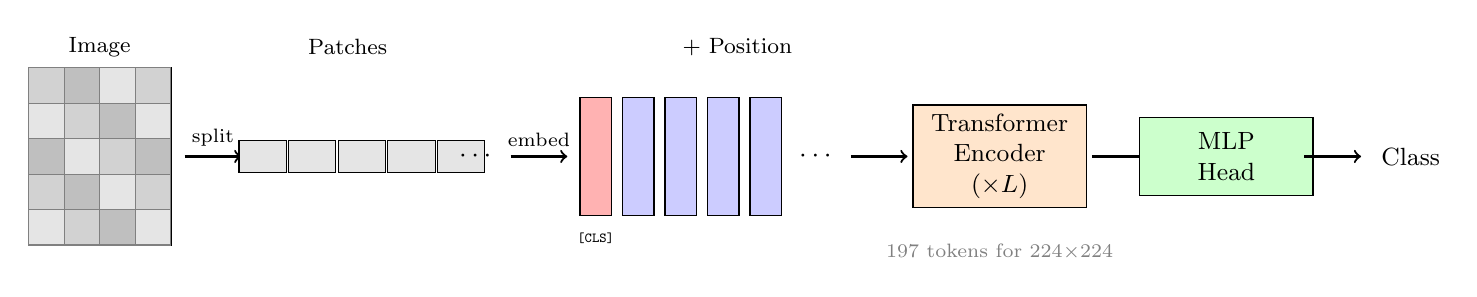
\begin{tikzpicture}[
        patch/.style={rectangle, draw, minimum size=0.5cm, fill=gray!20},
        emb/.style={rectangle, draw, fill=blue!20, minimum width=0.4cm, minimum height=1.5cm},
        cls/.style={rectangle, draw, fill=red!30, minimum width=0.4cm, minimum height=1.5cm},
        block/.style={rectangle, draw, minimum width=2.2cm, minimum height=1cm, align=center, font=\small},
        arrow/.style={->, thick},
        scale=0.9
    ]
        % Original image
        \node[font=\footnotesize] at (-5.5, 2.3) {Image};
        \draw[thick] (-6.5, -0.5) rectangle (-4.5, 2);

        % Grid showing patches
        \foreach \x in {0, 1, 2, 3} {
            \foreach \y in {0, 1, 2, 3, 4} {
                \pgfmathsetmacro{\shade}{20 + mod(\x + \y, 3) * 15}
                \fill[gray!\shade!white] (-6.5+\x*0.5, -0.5+\y*0.5) rectangle (-6.0+\x*0.5, 0+\y*0.5);
                \draw[gray, thin] (-6.5+\x*0.5, -0.5+\y*0.5) rectangle (-6.0+\x*0.5, 0+\y*0.5);
            }
        }

        % Arrow
        \draw[arrow] (-4.3, 0.75) -- (-3.5, 0.75);
        \node[font=\scriptsize, above] at (-3.9, 0.75) {split};

        % Flattened patches
        \node[font=\footnotesize] at (-2, 2.3) {Patches};
        \foreach \i in {0, 1, 2, 3, 4} {
            \node[patch, minimum width=0.6cm, minimum height=0.4cm] at (-3.2+\i*0.7, 0.75) {};
        }
        \node at (-0.2, 0.75) {$\cdots$};

        % Arrow
        \draw[arrow] (0.3, 0.75) -- (1.1, 0.75);
        \node[font=\scriptsize, above] at (0.7, 0.75) {embed};

        % Embeddings with class token
        \node[font=\footnotesize] at (3.5, 2.3) {+ Position};
        \node[cls] (cls) at (1.5, 0.75) {};
        \node[font=\tiny] at (1.5, -0.4) {\texttt{[CLS]}};
        \foreach \i in {1, 2, 3, 4} {
            \node[emb] at (1.5+\i*0.6, 0.75) {};
        }
        \node at (4.6, 0.75) {$\cdots$};

        % Transformer
        \draw[arrow] (5.1, 0.75) -- (5.9, 0.75);
        \node[block, fill=orange!20] (trans) at (7.2, 0.75) {Transformer\\Encoder\\($\times L$)};

        % MLP head
        \draw[arrow] (8.5, 0.75) -- (9.3, 0.75);
        \node[block, fill=green!20] (mlp) at (10.4, 0.75) {MLP\\Head};

        % Output
        \draw[arrow] (11.5, 0.75) -- (12.3, 0.75);
        \node[font=\small] at (13, 0.75) {Class};

        % Annotation
        \node[font=\scriptsize, gray] at (7.2, -0.6) {197 tokens for 224$\times$224};
    \end{tikzpicture}
    \caption{Vision Transformer (ViT) architecture. An image is divided into fixed-size patches (e.g., $16 \times 16$ pixels), which are flattened and projected to embeddings. A learnable \texttt{[CLS]} token is prepended, positional embeddings are added, and the sequence is processed by a standard Transformer encoder. The \texttt{[CLS]} token output is used for classification.}
    \label{fig:vit-architecture}
\end{figure}

\subsection{ViT Model Variants}

\begin{quickref}[ViT Model Sizes]
\begin{center}
\begin{tabular}{lcccccc}
\toprule
\textbf{Model} & \textbf{Layers} & \textbf{Hidden} & \textbf{MLP} & \textbf{Heads} & \textbf{Params} \\
\midrule
ViT-Base & 12 & 768 & 3072 & 12 & 86M \\
ViT-Large & 24 & 1024 & 4096 & 16 & 307M \\
ViT-Huge & 32 & 1280 & 5120 & 16 & 632M \\
\bottomrule
\end{tabular}
\end{center}

\textbf{Patch size variants:}
\begin{itemize}
    \item ViT-B/16: Base model with $16 \times 16$ patches (standard)
    \item ViT-B/32: Base model with $32 \times 32$ patches (faster, lower accuracy)
    \item ViT-B/14: Base model with $14 \times 14$ patches (slower, higher accuracy)
\end{itemize}

Smaller patches $\Rightarrow$ longer sequences $\Rightarrow$ more computation but finer-grained attention.
\end{quickref}

\subsection{Data Requirements and Inductive Bias}

\begin{redbox}
\textbf{ViT's Data Hunger}

Vision Transformers require \textbf{substantially more training data} than CNNs to achieve comparable performance.

\textbf{Experimental results (Dosovitskiy et al., 2020):}
\begin{center}
\begin{tabular}{lcc}
\toprule
\textbf{Pretraining Data} & \textbf{ViT-L/16} & \textbf{ResNet-152} \\
\midrule
ImageNet-1k (1.3M images) & 77.9\% & \textbf{79.6\%} \\
ImageNet-21k (14M images) & 83.6\% & 83.4\% \\
JFT-300M (300M images) & \textbf{87.8\%} & 86.4\% \\
\bottomrule
\end{tabular}
\end{center}

\textbf{Why the data requirement?}

CNNs have strong \textbf{inductive biases} built into their architecture:
\begin{itemize}
    \item \textbf{Locality:} Convolutional kernels process local regions; nearby pixels are assumed to be related
    \item \textbf{Translation equivariance:} The same kernel is applied everywhere; patterns are position-independent
    \item \textbf{Hierarchical features:} Deep CNNs build complex features from simple ones through pooling
\end{itemize}

Transformers have \textbf{no such biases}:
\begin{itemize}
    \item Self-attention treats all positions symmetrically
    \item No assumption that nearby patches are more related
    \item Must learn locality and translation patterns from data
\end{itemize}

\textbf{Trade-off:}
\begin{itemize}
    \item With limited data: CNN biases help generalisation
    \item With abundant data: Transformer flexibility allows learning more powerful representations
\end{itemize}

\textbf{Practical implication:} For most practitioners with limited labelled data, CNNs or hybrid models remain strong choices. ViT excels in large-scale pretraining scenarios.
\end{redbox}

\subsection{ViT Variants and Improvements}

\begin{quickref}[Vision Transformer Variants]
\textbf{DeiT} (Data-efficient Image Transformer, 2021):
\begin{itemize}
    \item Trains ViT effectively on ImageNet-1k (no external data)
    \item Key: Strong data augmentation and regularisation
    \item Knowledge distillation from CNN teacher
\end{itemize}

\textbf{Swin Transformer} (2021):
\begin{itemize}
    \item Hierarchical structure (like CNNs)
    \item Shifted window attention (local, not global)
    \item Reduces complexity from $O(n^2)$ to $O(n)$ for images
    \item Excellent for dense prediction tasks (segmentation, detection)
\end{itemize}

\textbf{DINO} (Self-Distillation with No Labels, 2021):
\begin{itemize}
    \item Self-supervised pretraining for ViT
    \item Learns excellent features without any labels
    \item Discovers object segmentation automatically
\end{itemize}

\textbf{BEiT} (BERT Pre-Training of Image Transformers, 2021):
\begin{itemize}
    \item Masked image modelling (analogous to BERT's MLM)
    \item Predicts visual tokens for masked patches
\end{itemize}

\textbf{MAE} (Masked Autoencoders, 2022):
\begin{itemize}
    \item Masks 75\% of patches (much more aggressive than BERT)
    \item Reconstructs masked pixels
    \item Highly efficient pretraining
\end{itemize}
\end{quickref}

%==============================================================================
\section{Computational Considerations}
\label{sec:computational}
%==============================================================================

Understanding the computational properties of Transformers is essential for practical deployment. The quadratic complexity of self-attention, while enabling powerful modelling, imposes significant constraints on sequence length and model size.

\begin{rigour}[Transformer Complexity Analysis]
For a Transformer layer with:
\begin{itemize}
    \item Sequence length: $n$
    \item Model dimension: $d_{\text{model}} = d$
    \item FFN hidden dimension: $d_{\text{ff}} = 4d$ (standard)
    \item Number of heads: $h$
\end{itemize}

\textbf{Self-attention complexity:}
\begin{itemize}
    \item Q, K, V projections: $3 \cdot O(n \cdot d^2)$
    \item Attention scores $\mathbf{Q} \mathbf{K}^\top$: $O(n^2 \cdot d)$
    \item Softmax: $O(n^2)$
    \item Weighted sum $\text{scores} \times \mathbf{V}$: $O(n^2 \cdot d)$
    \item Output projection: $O(n \cdot d^2)$
\end{itemize}

\textbf{FFN complexity:}
\begin{itemize}
    \item First linear ($d \rightarrow 4d$): $O(n \cdot d \cdot 4d) = O(n \cdot d^2)$
    \item Second linear ($4d \rightarrow d$): $O(n \cdot 4d \cdot d) = O(n \cdot d^2)$
\end{itemize}

\textbf{Total per layer:}
\[
O(n^2 \cdot d + n \cdot d^2)
\]

\textbf{Memory for attention:}
\begin{itemize}
    \item Attention matrix: $O(n^2)$ per head, $O(h \cdot n^2)$ total
    \item For backpropagation: Must store attention matrices for gradient computation
\end{itemize}

\textbf{Which term dominates?}
\begin{itemize}
    \item $n^2 \cdot d$ vs $n \cdot d^2$
    \item Attention dominates when $n > d$
    \item FFN dominates when $d > n$
\end{itemize}

For typical models ($d = 768$, $n = 512$): Both terms contribute significantly.

For long sequences ($n = 4096$, $d = 768$): Attention dominates.
\end{rigour}

\begin{quickref}[Practical Implications of Transformer Complexity]
\textbf{Context length limits:}
\begin{itemize}
    \item BERT: 512 tokens
    \item GPT-2: 1024 tokens
    \item GPT-3: 2048 tokens
    \item GPT-4: 8192 / 32768 tokens
    \item Claude: 100,000+ tokens (requires efficient attention)
\end{itemize}

\textbf{Memory is often the bottleneck:}

For a 12-layer, 12-head model with $n = 2048$ and 16-bit precision:
\begin{itemize}
    \item Attention matrices: $12 \times 12 \times 2048^2 \times 2$ bytes $\approx$ 1.2 GB
    \item This is just for attention-activations and gradients add more
\end{itemize}

\textbf{Efficient attention implementations:}
\begin{itemize}
    \item \textbf{Flash Attention:} Fuses operations to avoid materialising $n^2$ attention matrix; uses tiling and recomputation
    \item \textbf{xFormers:} Memory-efficient attention library
    \item \textbf{Ring Attention:} Distributes attention computation across devices
\end{itemize}

\textbf{Approximate attention methods:}
\begin{itemize}
    \item \textbf{Sparse attention:} Attend to subset of positions (BigBird, Longformer)
    \item \textbf{Linear attention:} Replace softmax with kernel approximation
    \item \textbf{Low-rank attention:} Approximate attention matrix with low-rank factorisation
\end{itemize}
\end{quickref}

%==============================================================================
\section{Summary and Key Takeaways}
\label{sec:summary}
%==============================================================================

This chapter has traced the development from the information bottleneck problem in sequence-to-sequence learning through the attention mechanism to the Transformer architecture that now dominates deep learning.

\begin{quickref}[Chapter Summary]
\textbf{The Problem: Information Bottleneck}
\begin{itemize}
    \item Encoder-decoder models compress variable-length inputs to fixed-size context
    \item For long sequences, information is lost in this compression
    \item The decoder cannot selectively focus on relevant input positions
\end{itemize}

\textbf{The Solution: Attention}
\begin{itemize}
    \item Compute a \textit{different} context vector for each output position
    \item Context is a weighted combination of encoder states
    \item Weights determined by query-key compatibility (soft alignment)
\end{itemize}

\textbf{Key Attention Mechanisms:}
\begin{itemize}
    \item \textbf{Bahdanau attention:} Dynamic context for encoder-decoder; uses additive scoring
    \item \textbf{Scaled dot-product attention:} Efficient scoring via $\frac{\mathbf{Q}\mathbf{K}^\top}{\sqrt{d}}$; scaling prevents softmax saturation
    \item \textbf{Multi-head attention:} Parallel attention in different subspaces; captures diverse patterns
    \item \textbf{Self-attention:} Sequence attends to itself; $O(1)$ path length for any pair of positions
\end{itemize}

\textbf{The Transformer:}
\begin{itemize}
    \item Built entirely on attention (no recurrence, no convolution)
    \item Encoder: Self-attention + FFN with residuals and layer norm
    \item Decoder: Masked self-attention + cross-attention + FFN
    \item Positional encoding injects position information
\end{itemize}

\textbf{Architecture Variants:}
\begin{itemize}
    \item \textbf{Encoder-decoder:} Translation, summarisation (T5, BART)
    \item \textbf{Encoder-only:} Understanding tasks (BERT)
    \item \textbf{Decoder-only:} Generation (GPT, LLaMA, Claude)
\end{itemize}

\textbf{Pretrained Models:}
\begin{itemize}
    \item \textbf{BERT:} Bidirectional encoder; masked language modelling; pretrain then fine-tune paradigm
    \item \textbf{ViT:} Images as patch sequences; powerful but data-hungry
\end{itemize}

\textbf{Computational Considerations:}
\begin{itemize}
    \item Self-attention: $O(n^2)$ complexity in sequence length
    \item Memory for attention matrices often the bottleneck
    \item Efficient implementations (Flash Attention) and sparse approximations enable longer contexts
\end{itemize}
\end{quickref}

\begin{quickref}[Key Equations]
\textbf{Scaled dot-product attention:}
\[
\text{Attention}(\mathbf{Q}, \mathbf{K}, \mathbf{V}) = \text{softmax}\left(\frac{\mathbf{Q}\mathbf{K}^\top}{\sqrt{d_k}}\right)\mathbf{V}
\]

\textbf{Multi-head attention:}
\[
\text{MultiHead}(\mathbf{Q}, \mathbf{K}, \mathbf{V}) = \text{Concat}(\text{head}_1, \ldots, \text{head}_h)\mathbf{W}^O
\]

\textbf{Bahdanau context vector:}
\[
\mathbf{c}_{t'} = \sum_{t=1}^{T} \alpha(\mathbf{s}_{t'-1}, \mathbf{h}_t) \, \mathbf{h}_t
\]

\textbf{Self-attention output (position $i$):}
\[
\mathbf{y}_i = \sum_{j=1}^{n} \text{softmax}\left(\frac{\mathbf{q}_i^\top \mathbf{k}_j}{\sqrt{d_k}}\right) \mathbf{v}_j
\]

\textbf{Sinusoidal positional encoding:}
\[
\text{PE}(\text{pos}, 2i) = \sin\left(\frac{\text{pos}}{10000^{2i/d}}\right), \quad \text{PE}(\text{pos}, 2i+1) = \cos\left(\frac{\text{pos}}{10000^{2i/d}}\right)
\]
\end{quickref}

\begin{redbox}
\textbf{Key Caveats and Limitations}

\textbf{1. Quadratic complexity:} Self-attention scales as $O(n^2)$, limiting context length. Very long documents require efficient attention variants.

\textbf{2. No inherent position awareness:} Transformers need explicit positional encoding; the choice of encoding affects extrapolation to longer sequences.

\textbf{3. Data requirements:} Transformers often need more data than CNNs or RNNs to learn comparable representations, especially for structured domains like vision.

\textbf{4. Interpretability is limited:} While attention weights provide some insight, they do not always reflect ``true'' importance; careful analysis is needed.

\textbf{5. Teacher forcing mismatch:} For autoregressive models, the train-test discrepancy (exposure bias) remains a challenge.
\end{redbox}

%==============================================================================
\section{Connections to Other Topics}
\label{sec:connections}
%==============================================================================

\begin{quickref}[Cross-References and Connections]
\textbf{Building on previous chapters:}
\begin{itemize}
    \item \textbf{Chapter~\ref{ch:week6} (RNNs and LSTMs):} The encoder-decoder architecture was originally RNN-based. Understanding RNN limitations (sequential processing, vanishing gradients, difficulty with long-range dependencies) motivates attention.
    \item \textbf{Chapter~\ref{ch:week7} (Word Embeddings):} Token embeddings (Word2Vec, GloVe) provide input representations. BERT produces \textit{contextualised} embeddings-different representations for the same word in different contexts.
    \item \textbf{Chapter~\ref{ch:week5} (Regularisation and Optimisation):} Residual connections (crucial for deep Transformers) and dropout (applied in attention and FFN) were covered there. Layer normalisation plays a similar role to batch normalisation.
\end{itemize}

\textbf{Architectural concepts:}
\begin{itemize}
    \item \textbf{Residual connections:} Enable training of deep Transformers (dozens of layers). Without residuals, gradient flow degrades.
    \item \textbf{Layer normalisation:} Stabilises training, especially important for attention where activations can have high variance.
\end{itemize}

\textbf{Looking ahead:}
\begin{itemize}
    \item Large language models (GPT-3, GPT-4, LLaMA) are decoder-only Transformers at massive scale
    \item Multimodal models (CLIP, Flamingo) extend Transformers to multiple modalities
    \item Reinforcement learning from human feedback (RLHF) fine-tunes pretrained Transformers for alignment
\end{itemize}

\textbf{Broader significance:}

The Transformer architecture has unified deep learning across modalities:
\begin{itemize}
    \item \textbf{Text:} GPT, BERT, T5, LLaMA
    \item \textbf{Images:} ViT, DINO, MAE
    \item \textbf{Audio:} Whisper, Wav2Vec 2.0
    \item \textbf{Video:} ViViT, Video Swin
    \item \textbf{Multimodal:} CLIP, Flamingo, GPT-4V
\end{itemize}

Understanding Transformers is now foundational for virtually all areas of deep learning.
\end{quickref}

%==============================================================================
% References
%==============================================================================

\begin{rigour}[Key References]
\textbf{Foundational papers:}
\begin{itemize}
    \item Vaswani et al.\ (2017), ``Attention Is All You Need''-introduced the Transformer
    \item Bahdanau et al.\ (2015), ``Neural Machine Translation by Jointly Learning to Align and Translate''-attention for seq2seq
    \item Devlin et al.\ (2019), ``BERT: Pre-training of Deep Bidirectional Transformers for Language Understanding''
    \item Dosovitskiy et al.\ (2020), ``An Image is Worth 16x16 Words: Transformers for Image Recognition at Scale''-ViT
\end{itemize}

\textbf{Textbook resources:}
\begin{itemize}
    \item Zhang et al., ``Dive into Deep Learning,'' Chapters 10--11 (attention and Transformers)
    \item Jurafsky \& Martin, ``Speech and Language Processing,'' Chapter 10 (Transformers)
\end{itemize}

\textbf{Subsequent developments:}
\begin{itemize}
    \item Liu et al.\ (2019), ``RoBERTa: A Robustly Optimized BERT Pretraining Approach''
    \item Radford et al.\ (2019), ``Language Models are Unsupervised Multitask Learners'' (GPT-2)
    \item Brown et al.\ (2020), ``Language Models are Few-Shot Learners'' (GPT-3)
    \item Touvron et al.\ (2023), ``LLaMA: Open and Efficient Foundation Language Models''
\end{itemize}
\end{rigour}
